\section{Rancangan Solusi}
\label{sec:rancangan-solusi}

Berdasarkan hasil analisis solusi pada Subbab \ref{sec:analisis-solusi}, rancangan solusi menjelaskan bentuk sistem yang dibangun. Fondasi DecMed, yaitu IOTA sebagai penyimpanan \textit{on-chain}, IPFS sebagai penyimpanan \textit{off-chain}, dan PRE sebagai mekanisme kriptografis pendukung distribusi akses, tetap dipertahankan.

\subsection{Rancangan Arsitektur Solusi}
\label{subsec:rancangan-arsitektur-solusi}

Arsitektur solusi mempertahankan tiga \textit{client} utama DecMed, yaitu \textit{Patient Client}, \textit{Hospital Client}, dan \textit{Ministry Client}. \textit{Patient Client} digunakan pasien untuk menerbitkan token akses awal. \textit{Hospital Client} digunakan oleh petugas administrasi, dokter, dan petugas laboratorium untuk mengakses atau memperbarui data sesuai kewenangannya. \textit{Ministry Client} tetap berada pada ruang lingkup manajemen fasyankes sebagaimana rancangan DecMed awal.

Perubahan utama berada pada \textit{server} PRE dan struktur token akses. Pada DecMed awal, token akses masih membawa informasi yang relatif terbatas, seperti \textit{address}, \textit{role}, dan \textit{purpose}. Pada rancangan ini, token tersebut diganti dengan Macaroon yang membawa daftar \textit{caveats}. Setiap \textit{request} akses data harus menyertakan Macaroon. \textit{Server} PRE kemudian memvalidasi keaslian token, mengevaluasi seluruh \textit{caveats}, memastikan bahwa permintaan akses sesuai dengan segmen data yang diminta, lalu menjalankan proses \textit{re-encryption} hanya jika semua pemeriksaan berhasil.

Gambaran arsitektur sistem secara keseluruhan dapat dilihat pada gambar X
% TODO: Gambar arsitektur solusi
, sedangkan rancangan penyimpanan \textit{on-chain} dan \textit{off-chain} dijelaskan pada Tabel X
dan Tabel Y
% TODO: Tabel skema penyimpanan on-chain dan off-chain
\subsection{Rancangan Segmentasi Data RME}
\label{subsec:rancangan-segmentasi-data-rme}

Sesuai dengan analisis solusi pada Subbab \ref{subsec:pemetaan-kebutuhan-solusi}, rancangan ini memecah data RME menjadi beberapa unit data terenkripsi berdasarkan kategori fungsi klinis sesuai dengan dokumen KMK \autocite{kemenkes1423-2022}. Agar segmentasi data dapat digunakan dalam mekanisme kontrol akses granular, setiap unit data perlu memiliki identitas kategori yang dapat dikenali secara konsisten oleh sistem. Identitas kategori tersebut digunakan pada proses validasi \textit{caveat}, pemfilteran data saat diambil dari penyimpanan \textit{on-chain}, serta pembatasan hak baca dan tulis berdasarkan konteks layanan kesehatan. Oleh karena itu, setiap data fungsi klinis direpresentasikan dalam bentuk \textit{category} yang digunakan secara konsisten pada metadata dan implementasi sistem.

Segmentasi diawali dengan mengikuti klasifikasi isi RME yang telah dibahas pada Subbab \ref{subsec:isi-rme}, yaitu dokumentasi administratif dan dokumentasi klinis. Isi RME kemudian dibagi berdasarkan \textit{dataset} seperti yang sudah dibahas pada Subbab \ref{subsec:analisis-segmentasi-data}. Terdapat empat \textit{dataset} klinis yang akan diimplementasikan pada rancangan ini. Masing-masing \textit{dataset} tersebut dipetakan menjadi satu \textit{dataset category} dan menjadi nilai pada \textit{enum} di implementasi.

Pada rancangan ini, istilah \textit{dataset category} digunakan untuk merepresentasikan kelompok dataset seperti rawat jalan atau laboratorium, sedangkan \textit{function category} merepresentasikan jenis fungsi klinis atau administratif di dalam masing-masing \textit{dataset}. Kombinasi kedua kategori tersebut membentuk unit segmentasi terkecil yang digunakan dalam proses kontrol akses.

Dokumentasi administratif tidak termasuk ke dalam \textit{dataset} klinis berdasarkan kategori fungsi klinis KMK. Namun, dokumentasi administratif tetap direpresentasikan sebagai \textit{dataset category} tersendiri agar kebutuhan akses administratif pada sistem tetap dapat dikelola secara konsisten. Hal ini berkaitan dengan kebutuhan fungsionalitas DecMed, khususnya kebutuhan fungsional dengan ID F01, F06, F07, F14, dan F21 pada Tabel di Lampiran \ref{tab:kebutuhan-fungsional-decmed} terpenuhi. Tabel pemetaan \textit{dataset category} dapat dilihat pada Tabel \ref{tab:mapping-dataset-category}

\begin{table}[!ht]
    \centering
    \caption{Tabel Pemetaan \textit{Dataset Category}}
    \label{tab:mapping-dataset-category}
    \small
    \begin{tabular}{|p{0.23\textwidth}|p{0.27\textwidth}|}
        \hline
        \textbf{\textit{Dataset Category}} & \textbf{\textit{Enum Value}} \\ \hline
        Administratif                      & \texttt{ADMINISTRATIVE}      \\ \hline
        Rawat Jalan                        & \texttt{RAWAT\_JALAN}        \\ \hline
        Rawat Inap                         & \texttt{RAWAT\_INAP}         \\ \hline
        Laboratorium                       & \texttt{LABORATORIUM}        \\ \hline
        Apotek                             & \texttt{APOTEK}              \\ \hline
    \end{tabular}
\end{table}

Setiap \textit{dataset category} kemudian dibagi berdasarkan kategori fungsi. Masing-masing kategori fungsi inilah yang kemudian dijadikan sebagai segmen terkecil dalam rancangan solusi segmentasi data. Kategori fungsi klinis tersebut dapat dilihat pada Lampiran \ref{lampiran:metadata-rme} untuk \textit{dataset} Rawat Jalan, Rawat Inap, Laboratorium, dan Apotek. Tabel \ref{tab:mapping-function-category} adalah pemetaan kategori fungsi klinis dan administratif yang akan digunakan pada implementasi.

\begin{table}[!ht]
    \centering
    \caption{Tabel Pemetaan \textit{Function Category}}
    \label{tab:mapping-function-category}
    \small
    \begin{tabular}{|p{0.35\textwidth}|p{0.45\textwidth}|}
        \hline
        \textbf{\textit{Function Category}} & \textbf{\textit{Enum Value}}                \\ \hline

        Anamnesis
                                            & \texttt{ANAMNESIS}
        \\ \hline

        Pemeriksaan Fisik
                                            & \texttt{PEMERIKSAAN\_FISIK}
        \\ \hline

        Pemeriksaan Psikologis, Sosial Ekonomi, Spiritual
                                            & \texttt{PEMERIKSAAN\_PSIKOLOGIS}
        \\ \hline

        Riwayat Penggunaan Obat
                                            & \texttt{RIWAYAT\_PENGGUNAAN\_OBAT}
        \\ \hline

        Rencana Rawat
                                            & \texttt{RENCANA\_RAWAT}
        \\ \hline

        Perencanaan Pemulangan Pasien
                                            & \texttt{PERENCANAAN\_PEMULANGAN}
        \\ \hline

        Instruksi Medik dan Keperawatan
                                            & \texttt{INSTRUKSI\_MEDIK\_DAN\_KEPERAWATAN}
        \\ \hline

        Pemeriksaan Penunjang
                                            & \texttt{PEMERIKSAAN\_PENUNJANG}
        \\ \hline

        Diagnosis
                                            & \texttt{DIAGNOSIS}
        \\ \hline

        \textit{Informed Consent}
                                            & \texttt{INFORMED\_CONSENT}
        \\ \hline

        Terapi
                                            & \texttt{TERAPI}
        \\ \hline

        Permintaan Pemeriksaan
                                            & \texttt{PERMINTAAN\_PEMERIKSAAN}
        \\ \hline

        Spesimen Klinis
                                            & \texttt{SPESIMEN\_KLINIS}
        \\ \hline

        Fiksasi dan Pengolahan Spesimen
                                            & \texttt{PENGOLAHAN\_SPESIMEN}
        \\ \hline

        Hasil Pemeriksaan
                                            & \texttt{HASIL\_PEMERIKSAAN}
        \\ \hline

        Interpretasi dan Validasi Hasil
                                            & \texttt{VALIDASI\_HASIL}
        \\ \hline

        Distribusi Hasil Pemeriksaan
                                            & \texttt{DISTRIBUSI\_HASIL}
        \\ \hline

        Data Resep dan Obat
                                            & \texttt{DATA\_RESEP\_DAN\_OBAT}
        \\ \hline

        Riwayat Alergi
                                            & \texttt{RIWAYAT\_ALERGI}
        \\ \hline

        Asal Resep
                                            & \texttt{ASAL\_RESEP}
        \\ \hline

        Dokter Penulis Resep
                                            & \texttt{DOKTER\_PENULIS\_RESEP}
        \\ \hline

        Status dan Pengkajian Resep
                                            & \texttt{STATUS\_DAN\_PENGKAJIAN\_RESEP}
        \\ \hline

        Status Resep
                                            & \texttt{STATUS\_RESEP}
        \\ \hline

        Waktu Penyiapan Obat
                                            & \texttt{WAKTU\_PENYIAPAN\_OBAT}
        \\ \hline

        Waktu Penyerahan Obat
                                            & \texttt{WAKTU\_PENYERAHAN\_OBAT}
        \\ \hline

        Nama Petugas yang Melakukan Dispensing
                                            & \texttt{PETUGAS\_DISPENSING}
        \\ \hline

        Etiket
                                            & \texttt{ETIKET}
        \\ \hline
    \end{tabular}
\end{table}

Setiap segmen data di IPFS memiliki CID dan metadata sendiri di IOTA. Metadata tersebut memuat informasi seperti \texttt{dataset\_category}, \texttt{ipfs\_cid}, \texttt{integrity\_hash}, serta kapsul kunci yang diperlukan oleh PRE. Dengan demikian, ketika seorang aktor meminta akses terhadap suatu segmen, \textit{server} PRE dapat mencocokkan \textit{caveats} pada token dengan metadata segmen data yang diminta. Apabila token hanya mengizinkan akses terhadap data laboratorium, maka token tersebut tidak dapat digunakan untuk meminta segmen riwayat klinis rawat jalan yang tidak relevan.

Pada skenario layanan kesehatan kolaboratif, segmentasi data ini menghasilkan pemisahan akses sebagai berikut.

\begin{enumerate}[leftmargin=*]
    \item Petugas administrasi mengakses segmen dokumentasi administratif saja.
    \item Dokter penanggung jawab pasien mengakses segmen dokumentasi klinis yang relevan, seperti rawat jalan.
    \item Petugas laboratorium mengakses segmen pemeriksaan penunjang dan menulis segmen hasil pemeriksaan saja tanpa membuka keseluruhan riwayat klinis pasien.
    \item Petugas apotek mengakses segmen data resep dan obat saja tanpa membuka keseluruhan riwayat klinis pasien.
    \item Perawat mengakses segmen anamnesis, pemeriksaan fisik, pemeriksaan psikologis dan instruksi medik dan keperawatan saja tanpa membuka keseluruhan riwayat klinis pasien.
\end{enumerate}

Rancangan ini menjadikan segmentasi penyimpanan sebagai prasyarat teknis bagi penegakan prinsip \textit{need-to-know}. Penyimpanan data pada sistem yang diusulkan dibagi menjadi dua lapisan. Lapisan \textit{on-chain} pada IOTA menyimpan metadata segmen yang diperlukan untuk penemuan data, validasi kategori akses, verifikasi integritas, dan pengelolaan kapsul kunci. Lapisan \textit{off-chain} pada IPFS menyimpan isi RME dalam bentuk segmen data terenkripsi. Pemisahan ini memungkinkan \textit{server} PRE mencocokkan \textit{caveats} pada Macaroon dengan metadata segmen sebelum mengambil dan melakukan \textit{re-encryption} terhadap data di IPFS.

\subsubsection{Skema Penyimpanan \textit{On-Chain} (IOTA)}
\label{subsubsec:skema-penyimpanan-onchain}

Penyimpanan \textit{on-chain} tidak menyimpan isi rekam medis. Data yang dicatat pada IOTA adalah metadata setiap segmen RME yang sudah terenkripsi di IPFS. Metadata ini menjadi dasar bagi proses pemfilteran berdasarkan \texttt{dataset\_category} dan \texttt{function\_category}, serta menjadi sumber verifikasi bahwa segmen yang diminta sesuai dengan batasan akses pada token Macaroon.

\begin{longtable}{|>{\raggedright\arraybackslash}p{2.8cm}|>{\raggedright\arraybackslash}p{4.0cm}|>{\raggedright\arraybackslash}p{5.4cm}|}
    \caption{Skema Metadata Segmen RME \textit{On-Chain}} \label{tab:onchain-schema}                                                              \\
    \hline
    \textbf{Komponen} & \textbf{Key JSON}                                                                                   & \textbf{Keterangan} \\
    \hline
    \endfirsthead
    \hline
    \textbf{Komponen} & \textbf{Key JSON}                                                                                   & \textbf{Keterangan} \\
    \hline
    \endhead

    \multirow{4}{2.8cm}{\textbf{Identitas Segmen}}
                      & \texttt{segment\_id}
                      & UUID unik untuk satu segmen data RME.                                                                                     \\ \cline{2-3}
                      & \texttt{related\_rme\_id}
                      & ID RME atau episode pelayanan yasng menjadi induk segmen.                                                                 \\ \cline{2-3}
                      & \texttt{patient\_address}
                      & Alamat \textit{wallet} pasien pemilik RME.                                                                                \\ \cline{2-3}
                      & \texttt{fasyankes\_id}
                      & ID fasilitas pelayanan kesehatan yang menyimpan segmen.                                                                   \\ \hline

    \multirow{2}{2.8cm}{\textbf{Kategori Akses}}
                      & \texttt{dataset\_category}
                      & Kategori dataset. Sesuai dengan tabel \ref{tab:mapping-dataset-category}.                                                 \\ \cline{2-3}
                      & \texttt{function\_category}
                      & Kategori fungsi klinis atau administratif. Sesuai dengan tabel \ref{tab:mapping-function-category}.                       \\ \hline

    \multirow{3}{2.8cm}{\textbf{Pointer dan Integritas}}
                      & \texttt{ipfs\_cid}
                      & CID IPFS dari segmen data terenkripsi.                                                                                    \\ \cline{2-3}
                      & \texttt{integrity\_hash}
                      & Hash SHA-256 dari segmen terenkripsi.                                                                                     \\ \hline

    \multirow{3}{2.8cm}{\textbf{Kapsul Kunci}}
                      & \texttt{capsule}
                      & Kapsul PRE yang diperlukan untuk proses \textit{re-encryption}.                                                           \\ \cline{2-3}
                      & \texttt{enc\_key\_and\_nonce}
                      & Kunci simetris dan \textit{nonce} yang sudah terenkripsi untuk membuka segmen data.                                       \\ \cline{2-3}
                      & \texttt{encryption\_algo}
                      & Algoritma enkripsi konten, misalnya \texttt{AES-256-GCM}.                                                                 \\ \hline

    \multirow{3}{2.8cm}{\textbf{Audit Metadata}}
                      & \texttt{created\_at}
                      & Waktu pembuatan metadata segmen.                                                                                          \\ \cline{2-3}
                      & \texttt{author\_address}
                      & Alamat \textit{wallet} aktor yang membuat atau memperbarui segmen.                                                        \\ \cline{2-3}
                      & \texttt{updated\_at}
                      & Waktu pembaruan terakhir apabila segmen diganti dengan CID baru.                                                          \\ \hline
\end{longtable}

\subsubsection{Skema Penyimpanan \textit{Off-Chain} (IPFS)}
\label{subsubsec:skema-penyimpanan-offchain}

Data \textit{off-chain} disimpan sebagai objek JSON per segmen sebelum dienkripsi dan diunggah ke IPFS. Setiap segmen merepresentasikan satu kombinasi \texttt{dataset\_category} dan \texttt{function\_category}. Dengan demikian, akses terhadap data dapat diberikan hanya pada segmen yang sesuai dengan kebutuhan aktor, misalnya petugas laboratorium hanya memperoleh segmen \texttt{LABORATORIUM} yang relevan tanpa membuka seluruh riwayat klinis pasien.

\begin{longtable}{|>{\raggedright\arraybackslash}p{2.8cm}|>{\raggedright\arraybackslash}p{4.0cm}|>{\raggedright\arraybackslash}p{5.4cm}|}
    \caption{Skema Segmen Data RME \textit{Off-Chain}} \label{tab:offchain-schema}                                                                                                                                                  \\
    \hline
    \textbf{Komponen} & \textbf{Key JSON}                                                                                                                                                                     & \textbf{Keterangan} \\
    \hline
    \endfirsthead
    \hline
    \textbf{Komponen} & \textbf{Key JSON}                                                                                                                                                                     & \textbf{Keterangan} \\
    \hline
    \endhead

    \multirow{5}{2.8cm}{\textbf{Header Segmen}}
                      & \texttt{segment\_id}
                      & UUID yang sama dengan \texttt{segment\_id} pada metadata \textit{on-chain}.                                                                                                                                 \\ \cline{2-3}
                      & \texttt{related\_rme\_id}
                      & ID RME atau episode pelayanan yang menjadi induk segmen.                                                                                                                                                    \\ \cline{2-3}
                      & \texttt{dataset\_category}
                      & Kategori dataset sesuai Tabel \ref{tab:mapping-dataset-category}.                                                                                                                                           \\ \cline{2-3}
                      & \texttt{function\_category}
                      & Kategori fungsi sesuai dengan Tabel \ref{tab:mapping-function-category}. Untuk dokumentasi administratif yang tidak dirinci, nilai ini dapat menggunakan kategori administratif umum.                       \\ \hline

    \multirow{4}{2.8cm}{\textbf{Konteks Medis}}
                      & \texttt{patient\_ref}
                      & Identitas internal pasien yang diperlukan di dalam data terenkripsi.                                                                                                                                        \\ \cline{2-3}
                      & \texttt{encounter\_id}
                      & ID kunjungan atau episode pelayanan.                                                                                                                                                                        \\ \cline{2-3}
                      & \texttt{service\_date}
                      & Tanggal layanan, pemeriksaan, atau pembuatan segmen.                                                                                                                                                        \\ \cline{2-3}
                      & \texttt{author\_address}
                      & Alamat \textit{wallet} aktor yang menulis isi segmen.                                                                                                                                                       \\ \hline

    \multirow{2}{2.8cm}{\textbf{Isi Segmen}}
                      & \texttt{payload}
                      & Objek data RME sesuai kategori fungsi. Contoh isi dapat berupa data anamnesis, diagnosis, permintaan pemeriksaan, hasil laboratorium, atau data resep.                                                      \\ \cline{2-3}
                      & \texttt{payload\_hash}
                      & Hash isi \texttt{payload}.                                                                                                                                                                                  \\ \hline

    \multirow{3}{2.8cm}{\textbf{Lampiran Opsional}}
                      & \texttt{attachments[].cid}
                      & CID IPFS untuk lampiran terenkripsi yang terkait dengan segmen.                                                                                                                                             \\ \cline{2-3}
                      & \texttt{attachments[].\newline file\_name}
                      & Nama berkas lampiran.                                                                                                                                                                                       \\ \cline{2-3}
                      & \texttt{attachments[].\newline mime\_type}
                      & Jenis media lampiran, misalnya \texttt{application/pdf} atau \texttt{image/png}.                                                                                                                            \\ \hline
\end{longtable}

Secara konseptual, satu entri metadata \textit{on-chain} selalu menunjuk pada satu segmen terenkripsi \textit{off-chain}. Karena relasi ini dibuat per segmen, penegakan akses tidak lagi dilakukan terhadap satu \textit{encrypted blob} besar, melainkan terhadap unit data yang lebih kecil dan sesuai dengan kategori yang dinyatakan pada token Macaroon.

\subsection{Rancangan Model PBAC pada DecMed}
\label{subsec:rancangan-model-pbac-decmed}

Subbab ini merumuskan \textit{policy} akses atas objek. Berdasarkan analisis pada Subbab \ref{subsec:analisis-pendekatan-model-pbac}, elemen dan relasi \textit{Policy Machine} diadaptasi untuk memodelkan hubungan antara pengguna, atribut pengguna, segmen RME, atribut segmen, dan hak akses. Definisi formal pada subbab ini menjadi sumber kanonik bagi representasi \textit{caveat} Macaroon dan evaluasi pada \textit{Server} PRE.

Elemen \textit{policy} pada DecMed didefinisikan sebagai:

\begin{equation}
    PE_{\text{DecMed}}
    =
    U \cup UA \cup O \cup OA \cup PC,
\end{equation}

dengan [$U$] himpunan pengguna, [$UA$] himpunan atribut pengguna, [$O$] himpunan objek yang dilindungi, [$OA$] himpunan atribut objek, dan [$PC$] himpunan kelas \textit{policy}. Berdasarkan elemen tersebut, model \textit{policy} pada DecMed dirumuskan sebagai:

\begin{equation}
    PM_{\text{DecMed}}
    =
    \langle
    PE_{\text{DecMed}},
    AR,
    ASSIGN,
    ASSOCIATION,
    \mathcal{C}
    \rangle,
\end{equation}

dengan $AR$ sebagai himpunan hak akses, $ASSIGN$ sebagai relasi penugasan, $ASSOCIATION$ sebagai relasi asosiasi hak akses, dan $\mathcal{C}$ sebagai himpunan kondisi akses DecMed.

Elemen $\mathcal{C}$ merupakan perluasan pada rancangan ini untuk merepresentasikan kondisi dinamis yang ditegakkan melalui Macaroon dan \textit{Server} PRE, seperti masa berlaku, rantai delegasi, revokasi, dan bukti kepemilikan identitas aktor pada rantai delegasi.

\subsubsection{Pengguna dan Atribut Pengguna}

Himpunan pengguna $U$ berisi pengguna DecMed yaitu:

\begin{equation}
    U =
    {
    u_{\text{pasien}},
    u_{\text{petugas-rm}},
    u_{\text{perawat}},
    u_{\text{dokter}},
    u_{\text{laboratorium}},
    u_{\text{apoteker}}
    }.
\end{equation}

Elemen pada himpunan tersebut merepresentasikan alamat dompet aktual, bukan hanya nama peran. Sebagai contoh, $u_{\text{dokter-A}}$ dan $u_{\text{dokter-B}}$ merupakan dua pengguna yang berbeda meskipun keduanya memiliki atribut \textit{subrole} dokter. Atribut pengguna dibagi menjadi atribut kelembagaan dan atribut kapabilitas:

\begin{equation}
    UA = UA_{\text{role}} \cup UA_{\text{capability}}.
\end{equation}

Atribut kelembagaan menyatakan \textit{role} atau \textit{subrole} pengguna yang tercatat pada penyimpanan \textit{on-chain}:

\begin{equation}
    UA_{\text{role}} =
        {
            ua_{\text{patient}},
            ua_{\text{administrative-personnel}},
            ua_{\text{nurse}},
            ua_{\text{doctor}},
            ua_{\text{laboratory}},
            ua_{\text{pharmacist}}
        }.
\end{equation}

Relasi penugasan pengguna terhadap atribut perannya dinyatakan sebagai:

\begin{equation}
    u ; ASSIGN ; ua_{\operatorname{role}(u)}
\end{equation}

Atribut kapabilitas merupakan abstraksi terhadap kapabilitas efektif yang diperoleh dari suatu token Macaroon. Untuk token $\tau$, atribut kapabilitasnya dinyatakan sebagai:

\begin{equation}
    ua_{\operatorname{cap}(\tau)}
    \in UA_{\text{capability}}
\end{equation}

Atribut kapabilitas dibentuk secara konseptual ketika \textit{Server} PRE mengevaluasi token dan membentuk himpunan subjek dari \texttt{root\_subject} serta seluruh \texttt{delegated\_to} pada rantai delegasi. Pengguna hanya dianggap memiliki atribut kapabilitas apabila pengguna tersebut termasuk dalam himpunan subjek token dan dapat membuktikan kepemilikan \textit{wallet}:

\begin{equation}
    u ; ASSIGN ; ua_{\operatorname{cap}(\tau)}
    \iff
    \operatorname{ContainsSubject}(\tau,u)
    \land
    \operatorname{WalletProofValid}(u).
\end{equation}

Pemisahan atribut peran dan atribut kapabilitas diperlukan karena keduanya memiliki fungsi yang berbeda. Atribut kapabilitas menentukan cakupan data yang diberikan melalui token, sedangkan atribut peran menentukan apakah pengguna masih memiliki kewenangan kelembagaan yang sesuai. Dengan demikian, kepemilikan \textit{subrole} dokter tidak secara otomatis memberikan akses terhadap seluruh RME pasien.

\subsubsection{Objek dan Atribut Objek}

Himpunan objek $O$ terdiri atas segmen RME terenkripsi yang disimpan pada IPFS:

\begin{equation}
    O = {o_1,o_2,\ldots,o_n}.
\end{equation}

Setiap objek merepresentasikan satu segmen klinis. Informasi mengenai objek, seperti pasien, episode RME, kategori dataset, kategori fungsi, dan CID data terenkripsi, direpresentasikan melalui metadata pada IOTA.

Atribut objek $OA$ digunakan untuk mengelompokkan segmen berdasarkan beberapa tingkat yaitu:

\begin{enumerate}
    \item rumah sakit;
    \item pasien;
    \item episode RME;
    \item kategori dataset; dan
    \item kategori fungsi klinis.
\end{enumerate}

Contoh relasi penugasan untuk satu segmen diagnosis adalah:

\begin{equation}
    \begin{aligned}
        o_{\text{diagnosis-17}}
         & ; ASSIGN ;
        oa_{\text{diagnosis-RME-17}}   \\
         & ; ASSIGN ;
        oa_{\text{rawat-jalan-RME-17}} \\
         & ; ASSIGN ;
        oa_{\text{RME-17}}             \\
         & ; ASSIGN ;
        oa_{\text{pasien-P}}           \\
         & ; ASSIGN ;
        oa_{\text{rumah-sakit-H}}      \\
         & ; ASSIGN ;
        pc_{\text{DecMed}}.
    \end{aligned}
\end{equation}

Himpunan kategori dataset yang digunakan pada rancangan ini adalah $\texttt{RAWAT\_JALAN}$, $\texttt{RAWAT\_INAP}$, $\texttt{LABORATORIUM}$, dan $\texttt{APOTEK}$. Sementara itu, kategori fungsi mengikuti segmentasi data yang telah dijelaskan pada Subbab \ref{subsec:rancangan-segmentasi-data-rme}.

\subsubsection{Hak Akses dan Asosiasi}

Himpunan hak akses yang digunakan adalah:

\begin{equation}
    AR = {\texttt{Read},\texttt{Update}}.
\end{equation}

Hak \texttt{Read} menyatakan kemampuan membaca segmen RME, sedangkan hak \texttt{Update} menyatakan kemampuan menulis atau memperbarui segmen. Pada implementasi token, hak tersebut direpresentasikan melalui \textit{caveat} \texttt{purpose}. Cakupan objeknya direpresentasikan melalui \texttt{read\_dataset\_in}, \texttt{write\_dataset\_in}, \texttt{read\_function\_in}, dan \texttt{write\_function\_in}.

Pada \textit{Policy Machine}, asosiasi dinyatakan sebagai hubungan antara atribut pengguna, himpunan hak akses, dan atribut target:

\begin{equation}
    (ua, ars, oa) \in ASSOCIATION.
\end{equation}

Dalam rancangan DecMed, asosiasi dibentuk secara konseptual dari kapabilitas efektif token:

\begin{equation}
    \left(
    ua_{\operatorname{cap}(\tau)},
    AR_{\operatorname{eff}}(\tau),
    OA_{\operatorname{scope}}(\tau)
    \right)
    \in ASSOCIATION.
\end{equation}

$AR_{\operatorname{eff}}(\tau)$ merupakan hak akses efektif token, sedangkan $OA_{\operatorname{scope}}(\tau)$ merupakan himpunan atribut objek yang termasuk dalam cakupan token. Cakupan objek token didefinisikan sebagai:

\begin{equation}
    \begin{split}
        \operatorname{Scope}(\tau)
        =
        \{ o_s \in O \mid {} &
        p(s)=\operatorname{Patient}(\tau)                                 \\
                             & \land h(s)=\operatorname{Hospital}(\tau)   \\
                             & \land d(s)\in D_{\operatorname{eff}}(\tau) \\
                             & \land f(s)\in F_{\operatorname{eff}}(\tau) \\
                             & \land
        (
        \operatorname{Purpose}(\tau)=\texttt{Update}
        \Rightarrow
        r(s)=\operatorname{RME}(\tau)
        )
        \}.
    \end{split}
\end{equation}

$D_{\operatorname{eff}}(\tau)$ merupakan irisan seluruh \textit{caveats} \textit{dataset category} pada token, sedangkan $F_{\operatorname{eff}}(\tau)$ merupakan irisan seluruh \textit{caveats} \textit{function category}:

\begin{equation}
    D_{\operatorname{eff}}(\tau)
    =
    \bigcap_{i=1}^{n} D_i,
\end{equation}

\begin{equation}
    F_{\operatorname{eff}}(\tau)
    =
    \bigcap_{i=1}^{m} F_i.
\end{equation}

Penggunaan operasi irisan memastikan bahwa penambahan \textit{caveat} pada token turunan hanya dapat mempertahankan atau mempersempit cakupan akses. Penambahan \textit{caveat} baru tidak dapat mengembalikan \textit{dataset category} atau \textit{function category} yang telah dikecualikan oleh token induk.

Untuk operasi \texttt{Read}, token dapat digunakan terhadap seluruh episode RME pasien yang termasuk dalam kategori dataset dan fungsi yang diizinkan. Untuk operasi \texttt{Update}, cakupan juga harus sesuai dengan \texttt{related\_rme\_id} sehingga perubahan hanya dapat dilakukan terhadap episode pelayanan yang sedang menjadi konteks token.

\subsubsection{Kondisi \textit{Policy} Akses}

Selain asosiasi antara kapabilitas dan objek, keputusan akses juga dipengaruhi oleh himpunan kondisi $\mathcal{C}$. Kondisi yang digunakan pada DecMed ditunjukkan pada Tabel \ref{tab:pemetaan-kondisi-policy-decmed}.

\begin{table}[!ht]
    \centering
    \caption{Kondisi \textit{Policy} Akses DecMed}
    \label{tab:pemetaan-kondisi-policy-decmed}
    \small
    \begin{tabular}{|p{0.24\textwidth}|p{0.32\textwidth}|p{0.31\textwidth}|}
        \hline
        \textbf{Kondisi}
         & \textbf{Representasi}
         & \textbf{Fungsi}                                                            \\ \hline

        Identitas pasien
         & \texttt{patient\_address}
         & Membatasi token pada data milik pasien tertentu.                           \\ \hline

        Rumah sakit
         & \texttt{hospital\_cid}
         & Membatasi penggunaan token pada konteks rumah sakit tertentu.              \\ \hline

        Episode RME
         & \texttt{related\_rme\_id}
         & Membatasi operasi \texttt{Update} pada episode RME tertentu.               \\ \hline

        Subjek rantai delegasi
         & \texttt{root\_subject} dan seluruh \texttt{delegated\_to}
         & Menentukan himpunan alamat dompet yang berwenang menggunakan token.        \\ \hline

        Identitas aktor pemohon
         & \textit{Wallet proof}
         & Membuktikan bahwa permintaan ditandatangani oleh salah satu subjek rantai. \\ \hline

        Masa berlaku
         & \texttt{expires\_before}
         & Membatasi waktu penggunaan token.                                          \\ \hline

        Kedalaman delegasi
         & \texttt{max\_delegation\_depth} dan rantai delegasi
         & Membatasi jumlah penurunan token.                                          \\ \hline

        Hubungan token
         & \texttt{parent\_token\_hash}
         & Menghubungkan token turunan dengan token induk untuk revokasi.             \\ \hline

        Otoritas kelembagaan
         & \textit{Role} dan \textit{subrole} pada IOTA
         & Membatasi operasi tulis sesuai kewenangan tenaga kesehatan.                \\ \hline

        Status revokasi
         & Catatan revokasi
         & Menolak token awal atau token turunan yang telah dicabut.                  \\ \hline
    \end{tabular}

\end{table}

Masa berlaku efektif token merupakan nilai paling awal dari seluruh \textit{caveat} \texttt{expires\_before}:

\begin{equation}
    Expiry_{\operatorname{eff}}(\tau)
    =
    \min
    {
        Expiry_1,Expiry_2,\ldots,Expiry_n
    }.
\end{equation}

Himpunan subjek yang berwenang menggunakan token ditentukan berdasarkan rantai delegasi:

\begin{equation}
    \operatorname{Subjects}(\tau)
    =
    \left\{
    \operatorname{root\_subject}(\tau)
    \right\}
    \cup
    \left\{
    \operatorname{delegated\_to}_i(\tau)
    \mid
    1 \leq i \leq n
    \right\},
\end{equation}

dan permintaan dari aktor $u$ hanya diterima apabila:

\begin{equation}
    \operatorname{ContainsSubject}(\tau,u)
    \iff
    u \in \operatorname{Subjects}(\tau).
\end{equation}

Kedalaman delegasi dihitung berdasarkan jumlah perpindahan aktor pada rantai delegasi dan harus memenuhi:

\begin{equation}
    Depth(\tau)
    \leq
    MaxDepth(\tau).
\end{equation}

\subsubsection{Rancangan \textit{Policy} Delegasi}

Delegasi dimodelkan sebagai pembentukan kapabilitas turunan $\tau_c$ dari kapabilitas induk $\tau_p$. Token turunan hanya valid apabila tidak memperluas hak akses token induk.

Hubungan cakupan token harus memenuhi:

\begin{equation}
    \operatorname{Scope}(\tau_c)
    \subseteq
    \operatorname{Scope}(\tau_p).
\end{equation}

Hak akses token turunan juga harus memenuhi:

\begin{equation}
    AR_{\operatorname{eff}}(\tau_c)
    \subseteq
    AR_{\operatorname{eff}}(\tau_p).
\end{equation}

Batas waktu token turunan tidak boleh melebihi batas waktu token induk:

\begin{equation}
    Expiry_{\operatorname{eff}}(\tau_c)
    \leq
    Expiry_{\operatorname{eff}}(\tau_p).
\end{equation}

Selain itu, token turunan harus tetap berada dalam konteks pasien dan rumah sakit yang sama:

\begin{equation}
    Patient(\tau_c)=Patient(\tau_p),
\end{equation}

\begin{equation}
    Hospital(\tau_c)=Hospital(\tau_p).
\end{equation}

Untuk token dengan operasi \texttt{Update}, episode RME token turunan juga tidak boleh berbeda dari token induk:

\begin{equation}
    RME(\tau_c)=RME(\tau_p).
\end{equation}

Hubungan antara token turunan dan token induk disimpan melalui \texttt{parent\_token\_hash}. Sementara itu, perubahan aktor direpresentasikan dengan menambahkan \texttt{delegated\_by} dan \texttt{delegated\_to}. Karena seluruh \textit{caveat} token induk tetap dipertahankan, proses delegasi hanya dapat menambahkan \textit{caveats} baru dan tidak dapat menghapus \textit{caveats} sebelumnya.

\subsubsection{Fungsi Keputusan Akses}

Suatu permintaan akses terhadap segmen RME direpresentasikan sebagai:

\begin{equation}
    q =
    \langle
    u,h,p,r,d,f,a,t,\tau,\pi
    \rangle,
    \label{eq:permintaan-akses}
\end{equation}

dengan [$u$] alamat dompet pengguna yang melakukan permintaan, [$h$] identitas rumah sakit, [$p$] alamat pasien, [$r$] identitas episode RME, [$d$] kategori dataset, [$f$] kategori fungsi, [$a$] operasi yang diminta, [$t$] waktu permintaan, [$\tau$] token Macaroon, dan [$\pi$] bukti kepemilikan \textit{wallet}. Permintaan diberikan apabila seluruh kondisi \textit{policy} terpenuhi yaitu:

\begin{equation}
    \begin{split}
        \operatorname{Permit}(q)
        \iff {} &
        \operatorname{TokenValid}(\tau)                           \\
                & \land \operatorname{PurposeMatch}(a,\tau)       \\
                & \land \operatorname{ContainsSubject}(\tau,u)    \\
                & \land \operatorname{WalletProofValid}(\pi,q,u)  \\
                & \land \operatorname{PatientMatch}(p,\tau)       \\
                & \land \operatorname{HospitalMatch}(h,\tau)      \\
                & \land \operatorname{DatasetAllowed}(d,\tau)     \\
                & \land \operatorname{FunctionAllowed}(f,\tau)    \\
                & \land \operatorname{TimeValid}(t,\tau)          \\
                & \land \operatorname{DelegationChainValid}(\tau) \\
                & \land \neg\operatorname{Revoked}(\tau)
    \end{split}
    \label{eq:permit-akses}
\end{equation}

Apabila salah satu kondisi tidak terpenuhi, keputusan akses adalah:

\begin{equation}
    \operatorname{Decision}(q)=\operatorname{Deny}.
    \label{eq:deny-akses}
\end{equation}

Prinsip \textit{deny by default} diterapkan melalui fungsi tersebut. Kepemilikan token saja tidak cukup untuk memperoleh akses. Token harus valid, permintaan harus berasal dari salah satu aktor pada rantai delegasi, objek harus berada dalam cakupan token, token tidak boleh kedaluwarsa atau direvokasi, dan operasi tulis harus sesuai dengan \textit{subrole} tenaga kesehatan.

\subsubsection{Pemetaan Model \textit{Policy} ke Komponen DecMed}

Pemetaan elemen model \textit{policy} terhadap komponen implementasi ditunjukkan pada Tabel \ref{tab:pemetaan-policy-machine-decmed}.

\begin{table}[!ht]
    \centering
    \caption{Pemetaan Model \textit{Policy} terhadap Komponen DecMed}
    \label{tab:pemetaan-policy-machine-decmed}
    \small
    \begin{tabular}{|p{0.18\textwidth}|p{0.29\textwidth}|p{0.39\textwidth}|}
        \hline
        \textbf{Elemen}
         & \textbf{Representasi DecMed}
         & \textbf{Sumber atau Mekanisme Implementasi}                              \\ \hline

        $U$
         & Pengguna berdasarkan \textit{wallet address}
         & \textit{wallet address} dan tanda tangan \textit{wallet}.                \\ \hline

        $UA_{\text{role}}$
         & \textit{Role} dan \textit{subrole} pengguna
         & \textit{Registry Personnel} pada IOTA.                                   \\ \hline

        $UA_{\text{capability}}$
         & Kapabilitas efektif pengguna
         & Token Macaroon dan rantai delegasi.                                      \\ \hline

        $O$
         & Segmen RME terenkripsi
         & Objek data pada IPFS.                                                    \\ \hline

        $OA$
         & Rumah sakit, pasien, RME, dataset, dan fungsi
         & Metadata segmen pada IOTA.                                               \\ \hline

        $PC$
         & Kelas \textit{policy} DecMed
         & Aturan kontrol akses yang diberlakukan pada sistem DecMed.               \\ \hline

        $AR$
         & Operasi \texttt{Read} dan \texttt{Update}
         & \texttt{purpose} dan \textit{caveats} baca atau tulis pada Macaroon.     \\ \hline

        $ASSIGN$
         & Penugasan pengguna ke peran dan segmen ke kategori
         & Registri personel serta struktur metadata segmen.                        \\ \hline

        $ASSOCIATION$
         & Hubungan kapabilitas dengan hak dan cakupan objek
         & \textit{Effective capability} hasil evaluasi \textit{caveat}.            \\ \hline

        $\mathcal{C}$
         & Masa berlaku, delegasi, revokasi, dan bukti identitas
         & Macaroon, \textit{wallet proof}, Redis, IOTA, dan fungsi verifikasi PRE. \\ \hline
    \end{tabular}

\end{table}

Berdasarkan rancangan tersebut, model CapBAC yang telah digunakan oleh DecMed tidak digantikan oleh model PBAC. Macaroon tetap berfungsi sebagai token kapabilitas yang dibawa oleh pengguna, sedangkan elemen dan kondisi yang harus diperiksa untuk menafsirkan kapabilitas tersebut ditentukan oleh model PBAC. Dengan demikian, cara otoritas dibawa oleh token dijelaskan melalui CapBAC, sedangkan \textit{policy} yang menentukan validitas penggunaan otoritas tersebut dijelaskan melalui PBAC.

Rincian representasi \textit{policy} dalam bentuk \textit{caveat} dijelaskan pada Subbab \ref{subsec:rancangan-token-macaroons}. Mekanisme evaluasi dan penegakannya pada \textit{Server} PRE dijelaskan pada Subbab \ref{subsec:rancangan-penegakan-otoritas}.

\subsection{Rancangan Representasi Kebijakan pada Token Macaroons}
\label{subsec:rancangan-token-macaroons}

% Rancangan token otorisasi berbasis Macaroons pada subbab ini direferensikan sebagai \texttt{R-TA-04}. Rancangan ini merealisasikan \texttt{S-TA-03} untuk menjawab \texttt{M-TA-03} dan \texttt{M-TA-04}, serta merepresentasikan kapabilitas yang diturunkan dari model PBAC pada \texttt{R-TA-03}.

Berdasarkan model PBAC pada Subbab \ref{subsec:rancangan-model-pbac-decmed}, keputusan akses pada DecMed ditentukan berdasarkan hubungan antara pengguna, atribut pengguna, objek, atribut objek, hak akses, dan kondisi akses. Model tersebut masih berada pada tingkat konseptual sehingga membutuhkan representasi yang dapat dibawa oleh pengguna dan diverifikasi pada saat permintaan akses dilakukan.

Pada rancangan ini, Macaroon digunakan untuk merepresentasikan kapabilitas dan sebagian kondisi kebijakan akses. Token memuat identitas aktor yang berwenang menggunakan kapabilitas, cakupan objek yang dapat diakses, hak akses yang diberikan, masa berlaku, dan batasan delegasi. Namun, token tidak memuat seluruh keadaan kebijakan DecMed. Atribut kelembagaan pengguna, metadata objek, status revokasi, dan bukti kepemilikan alamat dompet diperoleh atau diverifikasi dari komponen sistem lain.

Dengan demikian, pembagian representasi kebijakan pada DecMed adalah sebagai berikut:

\begin{enumerate}
	\item Macaroon merepresentasikan atribut kapabilitas pengguna, hak akses, cakupan objek, masa berlaku, dan rantai delegasi.
	\item Penyimpanan \textit{on-chain} IOTA menyediakan atribut kelembagaan pengguna serta metadata pasien, rumah sakit, episode RME, kategori dataset, dan kategori fungsi dari objek.
	\item Redis menyediakan informasi yang diperlukan untuk memeriksa status revokasi token.
	\item Tanda tangan permintaan atau bukti kepemilikan \textit{wallet} mengikat penggunaan token dengan alamat dompet salah satu aktor pada rantai delegasi.
	\item \textit{Server} PRE menggabungkan seluruh informasi tersebut untuk menghasilkan keputusan \textit{permit} atau \textit{deny}.
\end{enumerate}

Macaroon tetap mengikuti model \textit{Capability-Based Access Control} karena token berfungsi sebagai bukti kapabilitas yang dibawa oleh pengguna. Sementara itu, aturan yang digunakan untuk menafsirkan dan memvalidasi kapabilitas tersebut ditentukan oleh model PBAC. Oleh karena itu, PBAC dan CapBAC tidak diposisikan sebagai dua pendekatan yang saling menggantikan. Kebijakan akses didefinisikan melalui PBAC, sedangkan Macaroon menjadi media pembawa kapabilitas yang dibatasi oleh kebijakan tersebut.

\subsubsection{Struktur Kapabilitas Efektif Token}

Sebuah token Macaroon $\tau$ secara konseptual terdiri atas identitas token, himpunan \textit{caveat}, dan tanda tangan autentikasi:

\begin{equation}
	\tau =
	\langle
	id_{\tau},
	C_{\tau},
	\sigma_{\tau}
	\rangle,
\end{equation}

dengan $id_{\tau}$ sebagai identitas token, $C_{\tau}$ sebagai himpunan \textit{caveat}, dan $\sigma_{\tau}$ sebagai tanda tangan Macaroon.

Himpunan \textit{caveat} pada token dievaluasi untuk membentuk kapabilitas efektif:

\begin{equation}
	\operatorname{Cap}_{\operatorname{eff}}(\tau)
	=
	\langle
	U_{\operatorname{subj}}(\tau),
	h,
	p,
	r,
	D_{\operatorname{eff}},
	F_{\operatorname{eff}},
	AR_{\operatorname{eff}},
	t_{\operatorname{exp}},
	depth
	\rangle,
\end{equation}

dengan:

\begin{description}
	\item[$U_{\operatorname{subj}}(\tau)$] himpunan aktor yang berwenang menggunakan token berdasarkan rantai delegasi;
	\item[$h$] rumah sakit yang menjadi konteks token;
	\item[$p$] pasien pemilik data;
	\item[$r$] episode RME yang dibatasi oleh token apabila berlaku;
	\item[$D_{\operatorname{eff}}$] himpunan kategori dataset efektif;
	\item[$F_{\operatorname{eff}}$] himpunan kategori fungsi efektif;
	\item[$AR_{\operatorname{eff}}$] hak akses efektif;
	\item[$t_{\operatorname{exp}}$] batas waktu efektif token; dan
	\item[$depth$] kedalaman rantai delegasi.
\end{description}

Kapabilitas efektif tersebut merupakan representasi dari atribut kapabilitas $ua_{\operatorname{cap}(\tau)}$ dan asosiasi hak akses yang telah didefinisikan pada Subbab \ref{subsec:rancangan-model-pbac-decmed}. Token tidak secara langsung menyimpan objek RME, tetapi menyimpan batasan yang akan dicocokkan dengan atribut objek pada metadata segmen.

\subsubsection{Pemetaan Elemen Kebijakan ke Caveat}

Pemetaan elemen kebijakan PBAC terhadap \textit{caveat} Macaroon ditunjukkan pada Tabel \ref{tab:pemetaan-policy-ke-caveat-macaroon}.

\begin{longtable}{|p{0.18\textwidth}|p{0.21\textwidth}|p{0.40\textwidth}|p{0.12\textwidth}|}
	\caption{Pemetaan Elemen Kebijakan ke \textit{Caveat} Macaroon}
	\label{tab:pemetaan-policy-ke-caveat-macaroon}                                              \\

	\hline
	\textbf{Elemen Kebijakan}
	 & \textbf{\textit{Caveat}}
	 & \textbf{Fungsi}
	 & \textbf{Token}                                                                           \\ \hline
	\endfirsthead

	\hline
	\textbf{Elemen Kebijakan}
	 & \textbf{\textit{Caveat}}
	 & \textbf{Fungsi}
	 & \textbf{Token}                                                                           \\ \hline
	\endhead

	Hak akses
	 & \texttt{purpose}
	 & Menyatakan operasi yang diizinkan, yaitu \texttt{Read} atau \texttt{Update}.
	 & Keduanya                                                                                 \\ \hline

	Atribut objek: pasien
	 & \texttt{patient\_\newline address}
	 & Membatasi kapabilitas terhadap RME milik pasien tertentu.
	 & Keduanya                                                                                 \\ \hline

	Atribut objek: rumah sakit
	 & \texttt{hospital\_cid}
	 & Membatasi penggunaan kapabilitas pada konteks rumah sakit tertentu.
	 & Keduanya                                                                                 \\ \hline

	Atribut objek: episode RME
	 & \texttt{related\_rme\_id}
	 & Membatasi operasi perubahan data pada satu episode RME.
	 & \texttt{Update}                                                                          \\ \hline

	Atribut kapabilitas: penerima awal
	 & \texttt{root\_subject}
	 & Menyatakan alamat dompet penerima token awal dari pasien.
	 & Keduanya                                                                                 \\ \hline

	Rantai delegasi
	 & \texttt{delegated\_by}
	 & Menyatakan alamat dompet aktor yang menurunkan token.
	 & Turunan                                                                                  \\ \hline

	Rantai delegasi
	 & \texttt{delegated\_to}
	 & Menyatakan alamat dompet penerima token turunan.
	 & Turunan                                                                                  \\ \hline

	Cakupan objek baca
	 & \texttt{read\_dataset\_\newline in}
	 & Membatasi kategori dataset yang dapat dibaca.
	 & \texttt{Read}                                                                            \\ \hline

	Cakupan objek tulis
	 & \texttt{write\_dataset\_\newline in}
	 & Membatasi kategori dataset yang dapat ditulis atau diperbarui.
	 & \texttt{Update}                                                                          \\ \hline

	Cakupan objek baca
	 & \texttt{read\_function\newline \_in}
	 & Membatasi kategori fungsi klinis yang dapat dibaca.
	 & \texttt{Read}                                                                            \\ \hline

	Cakupan objek tulis
	 & \texttt{write\_function\newline \_in}
	 & Membatasi kategori fungsi klinis yang dapat ditulis atau diperbarui.
	 & \texttt{Update}                                                                          \\ \hline

	Kondisi waktu
	 & \texttt{expires\_before}
	 & Menentukan batas waktu maksimum penggunaan kapabilitas.
	 & Keduanya                                                                                 \\ \hline

	Kondisi delegasi
	 & \texttt{max\_delegation\newline \_depth}
	 & Membatasi jumlah penurunan kapabilitas yang masih diizinkan.
	 & Keduanya                                                                                 \\ \hline

	Hubungan token
	 & \texttt{parent\_token\_\newline hash}
	 & Menghubungkan token turunan dengan token induknya untuk pemeriksaan rantai dan revokasi.
	 & Turunan                                                                                  \\ \hline
\end{longtable}

Nama \textit{caveat} \texttt{purpose} dipertahankan untuk menjaga kompatibilitas dengan implementasi DecMed sebelumnya. Namun, karena nilai yang digunakan adalah \texttt{Read} dan \texttt{Update}, secara semantik \textit{caveat} tersebut merepresentasikan hak akses $AR$.

\subsubsection{Pemisahan Kebijakan di Dalam dan di Luar Token}

Tidak seluruh elemen kebijakan disimpan sebagai \textit{caveat} agar token tidak menjadi satu-satunya sumber kebenaran mengenai kondisi pengguna dan objek. Pemetaan elemen kebijakan yang diperiksa dari luar token ditunjukkan pada Tabel \ref{tab:kebijakan-eksternal-macaroon}.

\begin{table}[!ht]
	\centering
	\caption{Elemen Kebijakan yang Diverifikasi di Luar Token}
	\label{tab:kebijakan-eksternal-macaroon}
	\small
	\begin{tabular}{|p{0.25\textwidth}|p{0.27\textwidth}|p{0.37\textwidth}|}
		\hline
		\textbf{Elemen}
		 & \textbf{Sumber}
		 & \textbf{Fungsi}                                                                                         \\ \hline

		\textit{Role} dan \textit{subrole}
		 & Registri personel pada IOTA
		 & Memastikan aktor masih mempunyai kewenangan kelembagaan yang sesuai dengan operasi dan kategori data.   \\ \hline

		Atribut objek
		 & Metadata segmen pada IOTA
		 & Menyediakan pasien, rumah sakit, episode RME, kategori dataset, dan kategori fungsi aktual dari segmen. \\ \hline

		Kepemilikan alamat dompet
		 & Tanda tangan permintaan atau \textit{wallet proof}
		 & Memastikan pemohon merupakan salah satu aktor yang tercatat pada rantai delegasi token.                 \\ \hline

		Status revokasi
		 & Redis dan hubungan \texttt{parent\_token\_hash}
		 & Memastikan token dan token induknya belum dicabut.                                                      \\ \hline

		Data terenkripsi
		 & IPFS dan material kunci PRE
		 & Memastikan data hanya dapat dipulihkan setelah kebijakan akses terpenuhi.                               \\ \hline
	\end{tabular}

\end{table}

\subsubsection{Rancangan Token Read dan Update}

Implementasi DecMed sebelumnya menggunakan dua token terpisah untuk operasi baca dan perubahan data. Pola tersebut dipertahankan untuk menjaga kompatibilitas dengan \textit{smart contract}, \textit{client}, penyimpanan metadata akses, dan \textit{Server} PRE.

Token baca memiliki:

\begin{equation}
	AR_{\operatorname{eff}}(\tau_{\operatorname{read}})
	=
	{\texttt{Read}},
\end{equation}

sedangkan token perubahan data memiliki:

\begin{equation}
	AR_{\operatorname{eff}}(\tau_{\operatorname{update}})
	=
	{\texttt{Update}}.
\end{equation}

Token baca menggunakan \texttt{read\_dataset\_in} dan \texttt{read\_function\_in}. Token perubahan data menggunakan \texttt{write\_dataset\_in} dan \texttt{write\_function\_in}. Pemisahan tersebut mencegah token baca digunakan sebagai dasar operasi tulis meskipun kategori dataset atau kategori fungsi yang diminta sama.

Pada token \texttt{Read}, \texttt{related\_rme\_id} tidak diwajibkan. Token baca dapat digunakan untuk membaca episode RME pasien yang berada pada rumah sakit, kategori dataset, dan kategori fungsi yang diizinkan. Dengan rancangan ini, kebutuhan tenaga medis, terutama dokter, untuk meninjau riwayat RME pasien ketika menentukan tindakan klinis didukung.

Pada token \texttt{Update}, \texttt{related\_rme\_id} wajib disertakan. Token tersebut hanya dapat digunakan untuk menulis atau memperbarui segmen pada episode pelayanan yang dinyatakan oleh \textit{caveat}. Pembatasan ini mencegah tenaga medis memperbarui episode RME lain hanya karena masih memiliki akses terhadap pasien yang sama.

Nilai \texttt{related\_rme\_id} menggunakan format \texttt{RME-\char`\{sequence\_6\_digit\char`\}}, misalnya \texttt{RME-000001}. Format tersebut mengikuti implementasi DecMed sebelumnya dan digunakan sebagai identitas episode RME pada prototipe.

\subsubsection{Rancangan Subjek Rantai Delegasi}

\textit{Caveat} \texttt{holder\_address} tidak digunakan pada rancangan token untuk menyatakan pemegang token tunggal. Hal ini disebabkan oleh sifat \textit{append-only} pada Macaroon. Apabila token awal memuat:

\begin{verbatim}
holder_address = 0xPETUGAS_REKAM_MEDIS
\end{verbatim}

kemudian token turunan menambahkan:

\begin{verbatim}
holder_address = 0xDOKTER
\end{verbatim}

maka token akan memiliki dua batasan identitas yang tidak dapat dipenuhi secara bersamaan. \textit{Caveat} lama tidak dapat dihapus atau diganti ketika token diturunkan.

Sebagai gantinya, aktor yang berwenang menggunakan token ditentukan dari rantai delegasi. \texttt{root\_subject} menyatakan aktor penerima token awal, sedangkan setiap proses delegasi menambahkan pasangan \texttt{delegated\_by} dan \texttt{delegated\_to}. Himpunan subjek token didefinisikan sebagai:

\begin{equation}
	\operatorname{Subjects}(\tau)
	=
	\left\{
	\operatorname{root\_subject}(\tau)
	\right\}
	\cup
	\left\{
	\operatorname{delegated\_to}_i(\tau)
	\mid
	1 \leq i \leq n
	\right\},
\end{equation}

dengan $n$ sebagai jumlah langkah delegasi pada token. Dengan demikian, seluruh aktor yang tercatat pada rantai delegasi berwenang menggunakan token tersebut, sepanjang mampu membuktikan kepemilikan \textit{wallet} masing-masing. Tanda tangan dari aktor di luar $\operatorname{Subjects}(\tau)$ ditolak.

Untuk setiap pasangan delegasi ke-$i$, rantai harus memenuhi:

\begin{equation}
	\operatorname{delegated\_by}_{i}
	=
	\begin{cases}
		\operatorname{root\_subject},
		 & i=1, \\
		\operatorname{delegated\_to}_{i-1},
		 & i>1.
	\end{cases}
\end{equation}

Pemeriksaan keanggotaan subjek dinyatakan sebagai:

\begin{equation}
	\operatorname{ContainsSubject}(\tau,u)
	\iff
	u \in \operatorname{Subjects}(\tau).
\end{equation}

\subsubsection{Penerbitan Token Awal}

Pada rancangan ini, \textit{Server} PRE bertindak sebagai penerbit token awal dan menyimpan \texttt{RootKey} yang digunakan untuk membentuk tanda tangan Macaroon. \texttt{RootKey} disimpan pada \textit{environment variable} \textit{Server} PRE dan tidak pernah diberikan kepada \textit{client}.

Token awal diterbitkan setelah alur pemberian akses oleh pasien telah terpenuhi. Pasien menentukan penerima awal, rumah sakit, cakupan kategori dataset, cakupan kategori fungsi, hak akses, masa berlaku, dan batas delegasi. Informasi tersebut menjadi dasar pembentukan \textit{caveat} pada token awal.

Alur penerbitan token awal adalah sebagai berikut:

\begin{enumerate}
	\item Pasien memilih aktor penerima dan cakupan akses.
	\item \textit{Client} pasien membentuk permintaan pemberian akses.
	\item \textit{Server} PRE memvalidasi identitas pasien dan parameter akses.
	\item \textit{Server} PRE membentuk token Macaroon menggunakan \texttt{RootKey}.
	\item Token dan metadata akses dicatat sesuai mekanisme pemberian akses DecMed.
	\item Token dapat digunakan oleh aktor yang ditentukan sebagai \texttt{root\_subject}.
\end{enumerate}

Pemisahan antara pasien dan penerbit token tidak menghilangkan sifat \textit{patient-centric}. Pasien tetap menjadi pihak yang menentukan pemberian akses awal, sedangkan \textit{Server} PRE menjalankan fungsi kriptografis untuk membentuk token yang dapat diverifikasi secara konsisten.

\subsubsection{Atenuasi Token sebagai Realisasi Delegasi}

Delegasi diwujudkan melalui pembentukan token turunan dengan penambahan \textit{caveat}. Pada rancangan ini, \textit{client} delegator tidak membentuk token turunan secara mandiri. \textit{Client} mengirimkan token induk, alamat penerima, cakupan yang diminta, masa berlaku, dan bukti identitas delegator kepada \textit{Server} PRE.

\textit{Server} PRE kemudian:

\begin{enumerate}
	\item memverifikasi tanda tangan dan seluruh \textit{caveat} token induk;
	\item membentuk himpunan subjek rantai delegasi token induk;
	\item memverifikasi bahwa permintaan berasal dari salah satu subjek pada rantai tersebut;
	\item memeriksa status revokasi token induk;
	\item memeriksa batas kedalaman delegasi;
	\item memastikan cakupan token turunan tidak melebihi token induk;
	\item menambahkan \texttt{delegated\_by}, \texttt{delegated\_to}, dan \texttt{parent\_token\_hash};
	\item menambahkan batasan dataset, fungsi, masa berlaku, atau kedalaman delegasi yang lebih sempit; dan
	\item menghasilkan token turunan.
\end{enumerate}

Token turunan $\tau_c$ dari token induk $\tau_p$ harus memenuhi:

\begin{equation}
	D_{\operatorname{eff}}(\tau_c)
	\subseteq
	D_{\operatorname{eff}}(\tau_p),
\end{equation}

\begin{equation}
	F_{\operatorname{eff}}(\tau_c)
	\subseteq
	F_{\operatorname{eff}}(\tau_p),
\end{equation}

\begin{equation}
	AR_{\operatorname{eff}}(\tau_c)
	\subseteq
	AR_{\operatorname{eff}}(\tau_p),
\end{equation}

dan:

\begin{equation}
	Expiry_{\operatorname{eff}}(\tau_c)
	\leq
	Expiry_{\operatorname{eff}}(\tau_p).
\end{equation}

Pasien dan rumah sakit pada token turunan tidak dapat diubah:

\begin{equation}
	Patient(\tau_c)=Patient(\tau_p),
\end{equation}

\begin{equation}
	Hospital(\tau_c)=Hospital(\tau_p).
\end{equation}

Untuk token \texttt{Update}, identitas episode RME juga harus tetap sama:

\begin{equation}
	RME(\tau_c)=RME(\tau_p).
\end{equation}

Sifat \textit{append-only} pada Macaroon memastikan seluruh \textit{caveat} token induk tetap terdapat pada token turunan. Nilai efektif dari batasan kategori dataset dan fungsi diperoleh melalui irisan seluruh batasan:

\begin{equation}
	D_{\operatorname{eff}}(\tau)
	=
	\bigcap_{i=1}^{n}D_i,
\end{equation}

\begin{equation}
	F_{\operatorname{eff}}(\tau)
	=
	\bigcap_{i=1}^{m}F_i.
\end{equation}

Batas waktu efektif diperoleh dari nilai paling awal:

\begin{equation}
	Expiry_{\operatorname{eff}}(\tau)
	=
	\min
	{
		Expiry_1,Expiry_2,\ldots,Expiry_n
	}.
\end{equation}

Dengan demikian, penambahan \textit{caveat} hanya dapat mempertahankan atau mempersempit kapabilitas. Token turunan tidak dapat menghapus batasan token induk untuk memperoleh cakupan akses yang lebih luas.

\subsubsection{Pembatasan Kedalaman dan Hubungan Token}

\textit{Caveat} \texttt{max\_delegation\_depth} menyatakan batas maksimum delegasi pada token. Kedalaman aktual dihitung dari jumlah pasangan \texttt{delegated\_by} dan \texttt{delegated\_to} pada rantai delegasi.

Token hanya dapat diturunkan apabila:

\begin{equation}
	Depth(\tau)
	<
	MaxDepth_{\operatorname{eff}}(\tau).
\end{equation}

Token turunan dapat menambahkan nilai \texttt{max\_delegation\_depth} yang lebih kecil untuk mengurangi kemampuan delegasi lebih lanjut. Nilai efektifnya diperoleh dari nilai minimum seluruh batasan kedalaman yang terdapat pada token.

\textit{Caveat} \texttt{parent\_token\_hash} hanya ditambahkan pada token turunan. Nilainya merupakan \textit{hash} token induk dan digunakan untuk membentuk hubungan antar-token. Hubungan tersebut mendukung pemeriksaan rantai delegasi dan mekanisme revokasi hierarkis.
% Rincian mekanisme revokasi dijelaskan pada Subbab \ref{subsubsec:revokasi-token-macaroons}.

\subsubsection{Penerapan Whitelisting dan Least Privilege}

Pendekatan \textit{whitelisting} digunakan untuk pembatasan kategori data. Token harus secara eksplisit mencantumkan kategori dataset dan kategori fungsi yang diizinkan. Kategori yang tidak dicantumkan dianggap tidak termasuk dalam cakupan token.

Pada token baca, sebuah segmen $o_s$ termasuk dalam cakupan apabila:

\begin{equation}
	\begin{split}
		o_s \in \operatorname{Scope}(\tau_{\operatorname{read}})
		\iff {} &
		p(s)=Patient(\tau)                                    \\
		        & \land h(s)=Hospital(\tau)                   \\
		        & \land d(s)\in D_{\operatorname{eff}}(\tau)  \\
		        & \land f(s)\in F_{\operatorname{eff}}(\tau).
	\end{split}
\end{equation}

Pada token perubahan data, syarat tersebut ditambah dengan kesesuaian episode RME:

\begin{equation}
	\begin{split}
		o_s \in \operatorname{Scope}(\tau_{\operatorname{update}})
		\iff {} &
		p(s)=Patient(\tau)                                    \\
		        & \land h(s)=Hospital(\tau)                   \\
		        & \land r(s)=RME(\tau)                        \\
		        & \land d(s)\in D_{\operatorname{eff}}(\tau)  \\
		        & \land f(s)\in F_{\operatorname{eff}}(\tau).
	\end{split}
\end{equation}

Prinsip \textit{least privilege} didukung oleh pendekatan ini. Dokter dapat memperoleh kapabilitas yang relatif luas sesuai kebutuhan pelayanan klinis, tetapi token turunan untuk petugas laboratorium atau apoteker dapat dibatasi hanya pada objek yang relevan.

Sebagai contoh, petugas laboratorium dapat memperoleh hak membaca fungsi \texttt{PEMERIKSAAN\_PENUNJANG} pada dataset \texttt{RAWAT\_JALAN} dan hak memperbarui fungsi \texttt{LABORATORIUM} pada dataset \texttt{LABORATORIUM}. Petugas tersebut tidak memperoleh akses terhadap anamnesis, diagnosis, terapi, resep, atau fungsi klinis lain yang tidak dicantumkan dalam token.

\subsubsection{Hubungan dengan Proses Verifikasi}

Token Macaroon bukan satu-satunya masukan keputusan akses. Pada saat token digunakan, \textit{Server} PRE membentuk kapabilitas efektif dengan memproses seluruh \textit{caveat}, kemudian mencocokkannya dengan permintaan, metadata objek, atribut pengguna, status revokasi, dan bukti kepemilikan \textit{wallet} dari aktor yang tercatat pada rantai delegasi.

Secara konseptual, penggunaan token hanya valid apabila:

\begin{equation}
	\begin{split}
		\operatorname{TokenUsable}(\tau,q)
		\iff {} &
		\operatorname{SignatureValid}(\tau)                        \\
		        & \land \operatorname{ContainsSubject}(\tau,u)     \\
		        & \land \operatorname{ObjectScopeMatch}(\tau,q)    \\
		        & \land \operatorname{AccessRightMatch}(\tau,q)    \\
		        & \land \operatorname{TimeValid}(\tau)             \\
		        & \land \operatorname{DelegationValid}(\tau)       \\
		        & \land \neg\operatorname{Revoked}(\tau)           \\
		        & \land \operatorname{ExternalAttributesValid}(q).
	\end{split}
	\label{eq:token-usable}
\end{equation}

$\operatorname{ExternalAttributesValid}(q)$ mencakup pemeriksaan \textit{role} atau \textit{subrole}, metadata segmen, dan bukti kepemilikan dompet. Rincian mekanisme penegakan tersebut dijelaskan pada Subbab \ref{subsec:rancangan-penegakan-otoritas}.

Contoh token awal untuk petugas rekam medis tetap disajikan pada Kode \ref{lst:contoh-token-baca-awal-rekam-medis} dan Kode \ref{lst:contoh-token-pembaruan-awal-rekam-medis}. Kedua contoh tersebut menunjukkan bagaimana kebijakan akses yang telah didefinisikan pada model PBAC direpresentasikan sebagai kumpulan \textit{caveat} yang dapat diverifikasi dan diatenuasi.

\subsection{Rancangan Penegakan Otoritas}
\label{subsec:rancangan-penegakan-otoritas}

% Rancangan penegakan otoritas pada subbab ini direferensikan sebagai \texttt{R-TA-05} untuk verifikasi \textit{caveats}, \textit{effective capability}, dan bukti kepemilikan \textit{wallet}, \texttt{R-TA-06} untuk validasi subrole tenaga medis terhadap dataset, serta \texttt{R-TA-07} untuk pencabutan akses token Macaroon delegasi. Rancangan ini merealisasikan \texttt{S-TA-04}, \texttt{S-TA-05}, dan \texttt{S-TA-06} untuk menjawab \texttt{M-TA-01}, \texttt{M-TA-02}, \texttt{M-TA-04}, \texttt{M-TA-05}, \texttt{M-TA-06}, dan \texttt{M-TA-07}.

Penegakan otoritas pada rancangan ini merujuk pada proses memastikan \textit{request} akses terhadap data RME hanya dilayani apabila aktor yang mengajukan permintaan memiliki kewenangan yang sah.

Bagian ini membahas tiga aspek utama penegakan otoritas pada \textit{Server} PRE. Pertama, Subbab \ref{subsubsec:verifikasi-caveats-macaroons-di-pre} menjelaskan verifikasi \textit{caveats} Macaroon untuk memastikan token masih valid. Kedua, Subbab \ref{subsubsec:verifikasi-role-tenaga-medis-untuk-akses-dataset} membahas validasi tambahan terhadap \textit{subrole} \texttt{MedicalPersonnel} agar akses tulis hanya dapat dilakukan pada \textit{dataset category} yang sesuai dengan kewenangannya. Ketiga, Subbab \ref{subsubsec:pencabutan-hak-akses-macaroon-delegasi} menjelaskan rancangan mekanisme revokasi token Macaroon, termasuk revokasi agar token turunannya tidak dapat digunakan.

Sebagai gambaran, Gambar \ref{fig:seqdiag-overview-penegakan-otoritas} menunjukkan alur penegakan otoritas pada \textit{Server} PRE. Secara garis besar, alur akses dimulai dengan aktor melalui \textit{client} untuk mengirimkan permintaan akses ke \textit{Server} PRE. \textit{Server} PRE kemudian memverifikasi token Macaroon, memverifikasi status revokasi dari token, dan menentukan aktor aktif. Jika semua verifikasi berhasil, \textit{Server} PRE melanjutkan proses ke 3 kemungkinan skenario, yaitu mengambil daftar RME yang dapat diakses, melakukan pembacaan data RME yang melibatkan proses \textit{re-encryption}, dan melakukan penulisan data RME.

\begin{figure}[!ht]
	\centering
	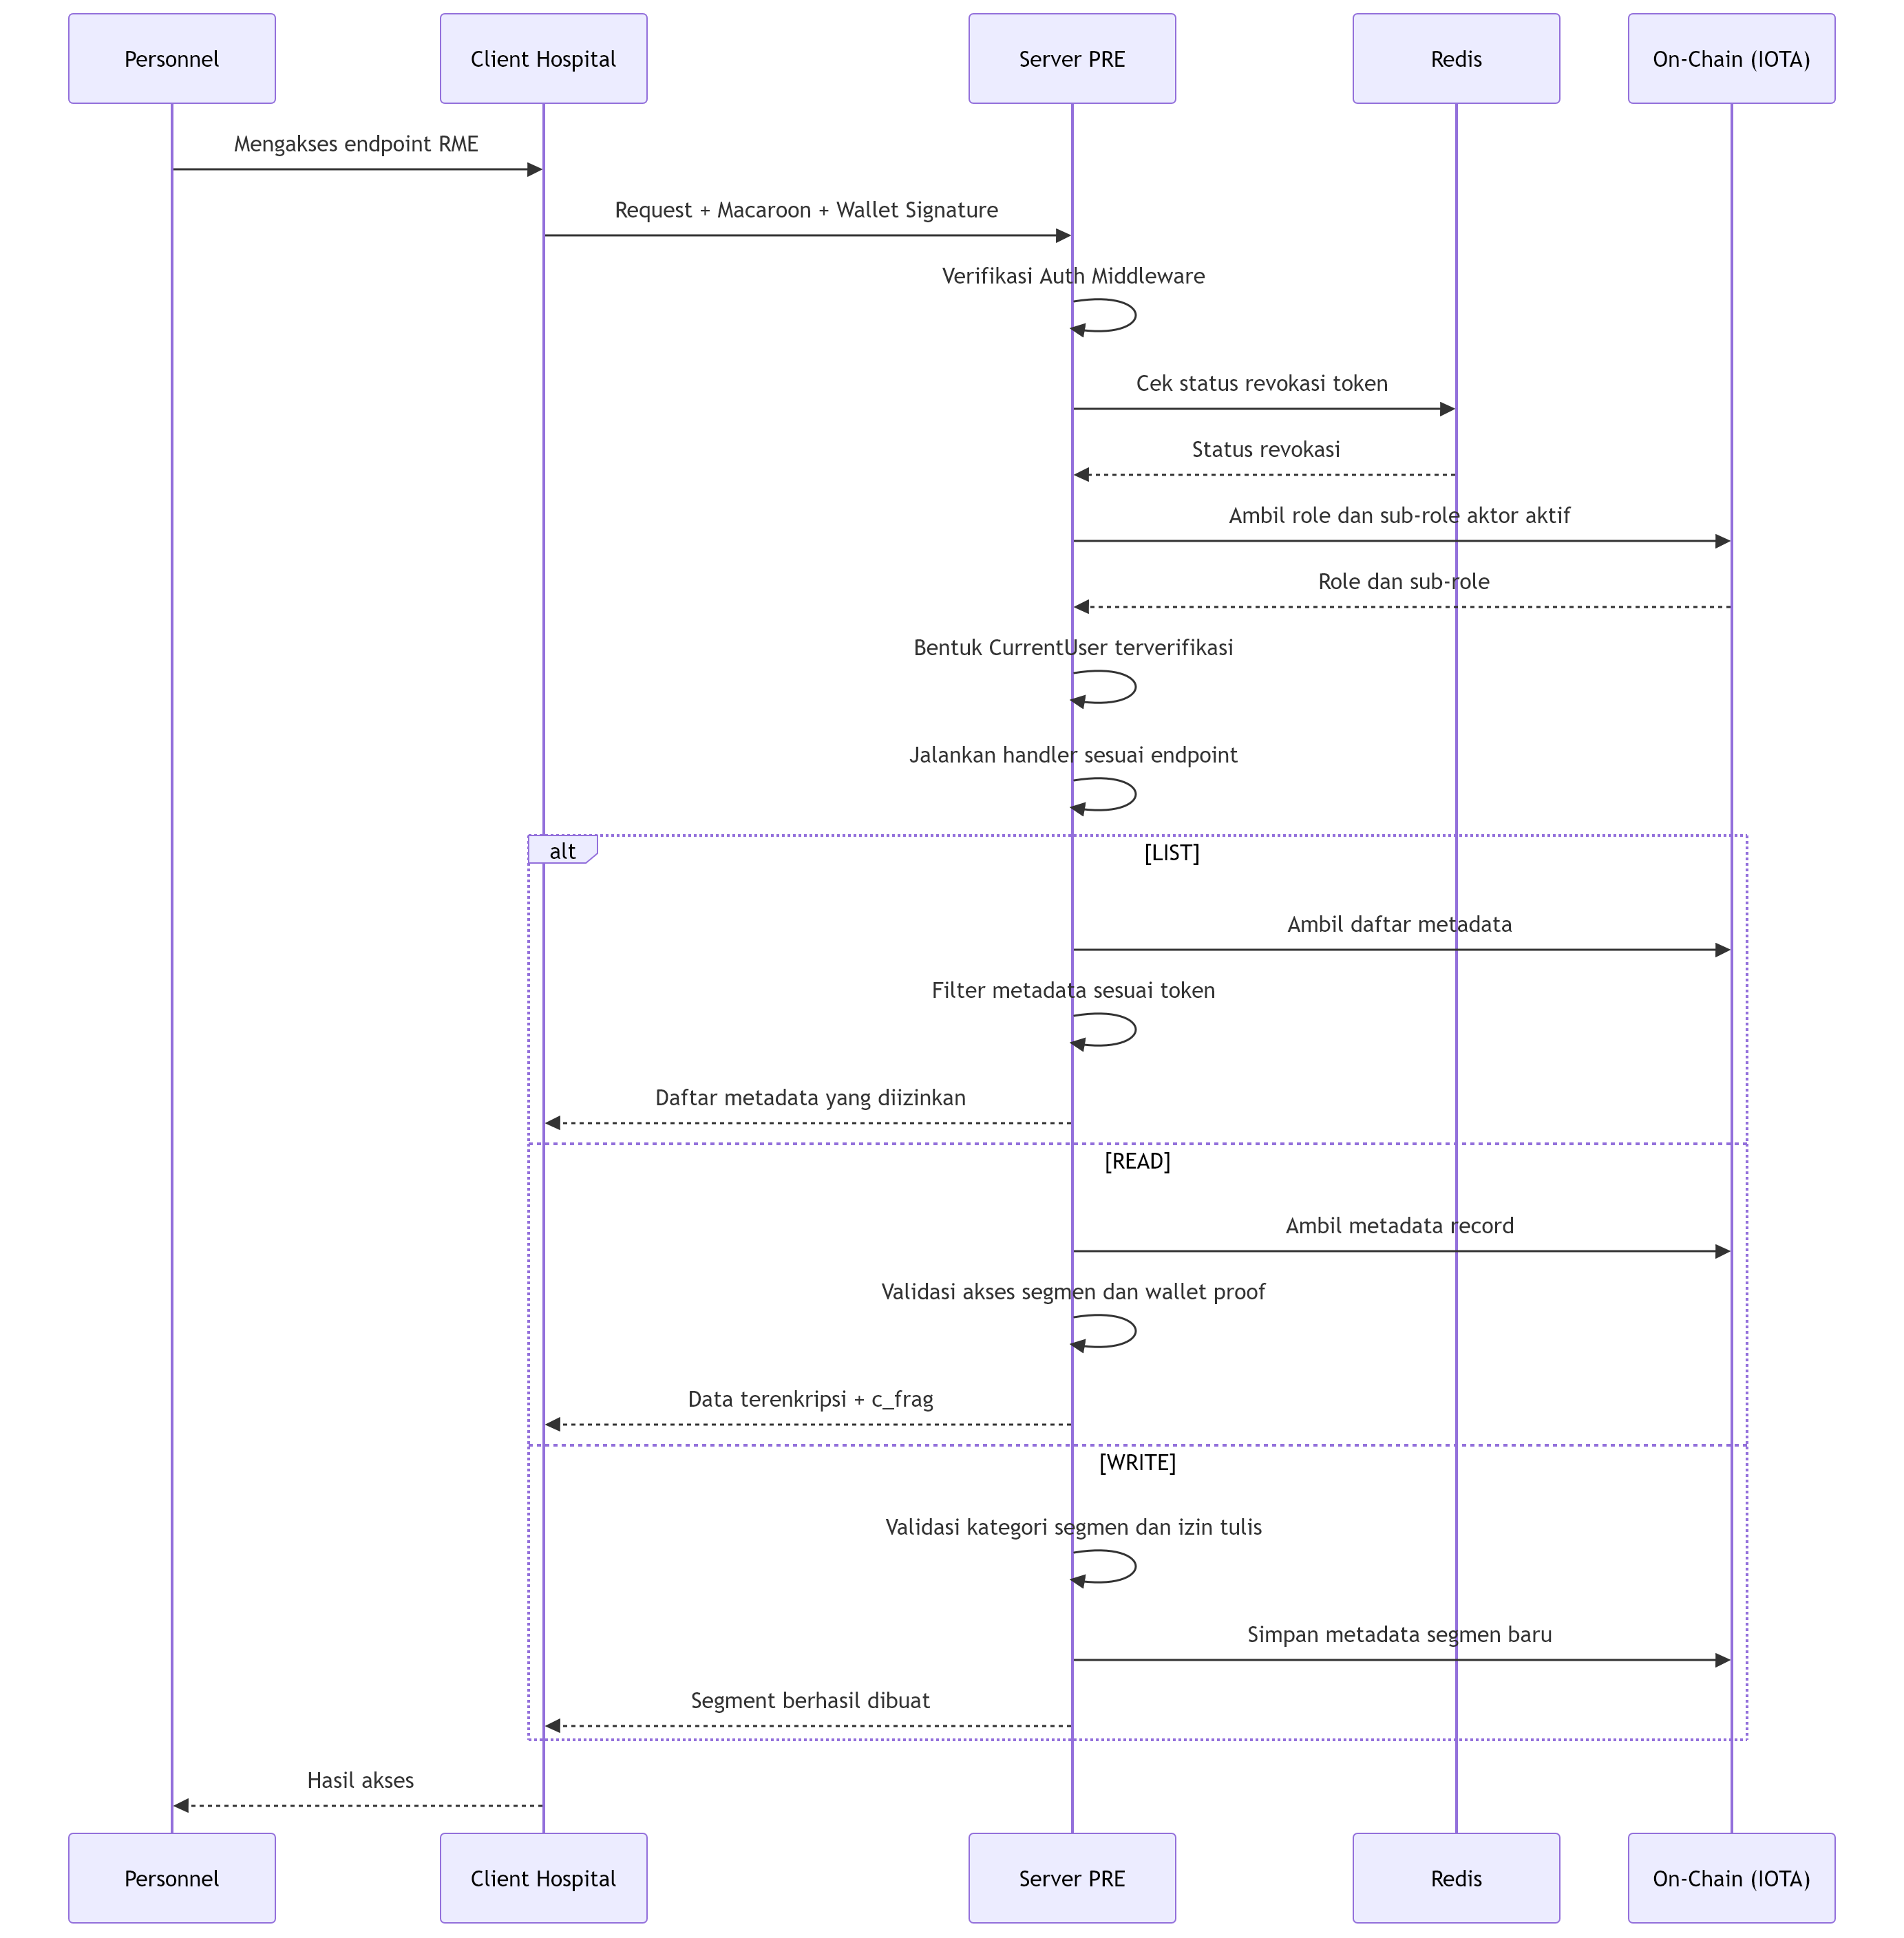
\includegraphics[width=\textwidth]{resources/chapter-3/rancangan/penegakan otoritas/seqdiag-overview.png}
	\caption{Alur penegakan otoritas pada \textit{Server} PRE}
	\label{fig:seqdiag-overview-penegakan-otoritas}
\end{figure}

\subsubsection{Verifikasi \textit{Caveats} Macaroons}
\label{subsubsec:verifikasi-caveats-macaroons-di-pre}

\textit{Server} PRE bertindak sebagai titik penegakan kebijakan akses. \textit{Server} PRE memverifikasi token Macaroon dan seluruh \textit{caveats}. Jika terdapat \textit{caveat} yang tidak dikenali atau diluar rancangan pada Tabel \ref{tab:rancangan-caveats-macaroons-baru}, permintaan akses ditolak.

Rancangan langkah verifikasi token Macaroon untuk permintaan akses baca data RME adalah sebagai berikut:

\begin{enumerate}[leftmargin=*]
	\item \textit{Server} PRE memverifikasi validitas token Macaroon melalui mekanisme \textit{Chained-HMAC} menggunakan \texttt{RootKey}.
	\item \textit{Server} PRE memverifikasi bahwa \texttt{patient\_address} dan \texttt{related\_rme\_id} pada token sesuai dengan data RME yang diminta.
	\item \textit{Server} PRE menghitung aktor aktif. Jika tidak terdapat \texttt{delegated\_to}, maka aktor aktif adalah \texttt{root\_subject}. Jika terdapat satu atau lebih \texttt{delegated\_to}, maka aktor aktif adalah nilai \texttt{delegated\_to} terakhir.
	\item \textit{Server} PRE memverifikasi tanda tangan \textit{wallet} dari aktor aktif pada permintaan akses.
	\item \textit{Server} PRE menghitung kedalaman delegasi berdasarkan jumlah \texttt{delegated\_to} pada token dan memastikan nilainya tidak melebihi \texttt{max\_delegation\_depth}.
	\item \textit{Server} PRE memvalidasi seluruh batas waktu pada \texttt{expires\_before} dan menggunakan batas waktu yang paling awal sebagai masa berlaku efektif token.
	\item \textit{Server} PRE menghitung cakupan akses efektif berdasarkan irisan seluruh \texttt{read\_dataset\_in}, \texttt{write\_dataset\_in}, \texttt{read\_function\_in}, dan \texttt{write\_function\_in}.
	\item \textit{Server} PRE mengambil metadata segmen dari IOTA dan mencocokkan \texttt{dataset\_category} serta \texttt{function\_category} segmen dengan cakupan akses efektif token.
	\item Jika seluruh verifikasi berhasil, \textit{Server} PRE melanjutkan proses pengambilan data terenkripsi dari IPFS dan melakukan \textit{re-encryption}. Jika salah satu pemeriksaan gagal, permintaan akses ditolak.
\end{enumerate}

\subsubsection{Verifikasi \textit{Role} dan \textit{Subrole} Tenaga Medis untuk Akses \textit{Dataset}}
\label{subsubsec:verifikasi-role-tenaga-medis-untuk-akses-dataset}

Dari hasil analisis pada Subbab \ref{subsec:analisis-verifikasi-aktor-operasi-tulis}, diperlukan verifikasi tambahan terhadap \textit{subrole} \texttt{MedicalPersonnel} agar akses tulis hanya dapat dilakukan pada \textit{dataset category} yang sesuai dengan kewenangannya. Pada implementasi Tugas Akhir ini, terdapat 4 \textit{subrole} turunan dari \textit{role} \texttt{MedicalPersonnel}, yaitu dokter, perawat, petugas laboratorium, dan apoteker. Sebagaimana dijelaskan pada Subbab \ref{subsec:analisis-segmentasi-data-rme}, setiap \textit{subrole} tersebut memiliki kebutuhan akses data yang berbeda-beda untuk melakukan akses jenis \textit{update}. Pemetaan kebutuhan akses data untuk setiap \textit{subrole} dapat dilihat pada Tabel \ref{tab:pemetaan-hak-akses-update-subrole}.

\begin{table}[!ht]
	\centering
	\caption{Pemetaan Hak Akses Update Berdasarkan subrole Tenaga Medis}
	\label{tab:pemetaan-hak-akses-update-subrole}
	\begin{tabular}{|p{0.15\textwidth}|p{0.35\textwidth}|p{0.35\textwidth}|}
		\hline
		\textbf{\textit{subrole}} & \textbf{\textit{Dataset Category}} & \textbf{\textit{Function Category}}                  \\
		\hline
		Perawat                   & Rawat Jalan/Rawat Inap             & Anamnesis, Pemeriksaan Fisik, Pemeriksaan Psikologis \\
		\hline
		Dokter                    & Rawat Jalan/Rawat Inap             & Seluruh \textit{function category}                   \\
		\hline
		Lab                       & Laboratorium                       & Laboratorium                                         \\
		\hline
		Apoteker                  & Apotek                             & Peresepan dan Dispensing                             \\
		\hline
	\end{tabular}
\end{table}

Berdasarkan pemetaan tersebut, terdapat verifikasi tambahan untuk \textit{role} \texttt{MedicalPersonnel}, yaitu melakukan validasi apakah \textit{subrole} pengguna yang saat ini mencoba melakukan aksi \textit{write} memang sesuai dengan jenis \textit{dataset} yang diakses. Alur tambahan tersebut ditunjukkan pada Gambar \ref{fig:seqdiag-validasi-subrole-dataset}. Pada alur ini, \textit{Server} PRE terlebih dahulu mendapatkan informasi \textit{subrole} tenaga medis melalui \textit{smart contract}. Informasi tersebut kemudian digunakan untuk memvalidasi pasangan \textit{role} dan \textit{subrole} terhadap kategori \textit{dataset} yang coba ditulis. Apabila \textit{subrole} aktor tidak memiliki kewenangan untuk menulis pada kategori \textit{dataset} tersebut, maka \textit{request} ditolak. Bagian berlatar merah pada Gambar \ref{fig:seqdiag-validasi-subrole-dataset} menunjukkan alur yang berubah atau ditambahkan pada rancangan Tugas Akhir ini dibandingkan Implementasi DecMed sebelumnya. Perubahan tersebut mencakup pengambilan informasi \textit{subrole} dari \textit{smart contract} serta validasi kesesuaian \textit{role}, \textit{subrole}, dan kategori \textit{dataset} sebelum akses tulis diberikan.

\begin{figure}[!ht]
	\centering
	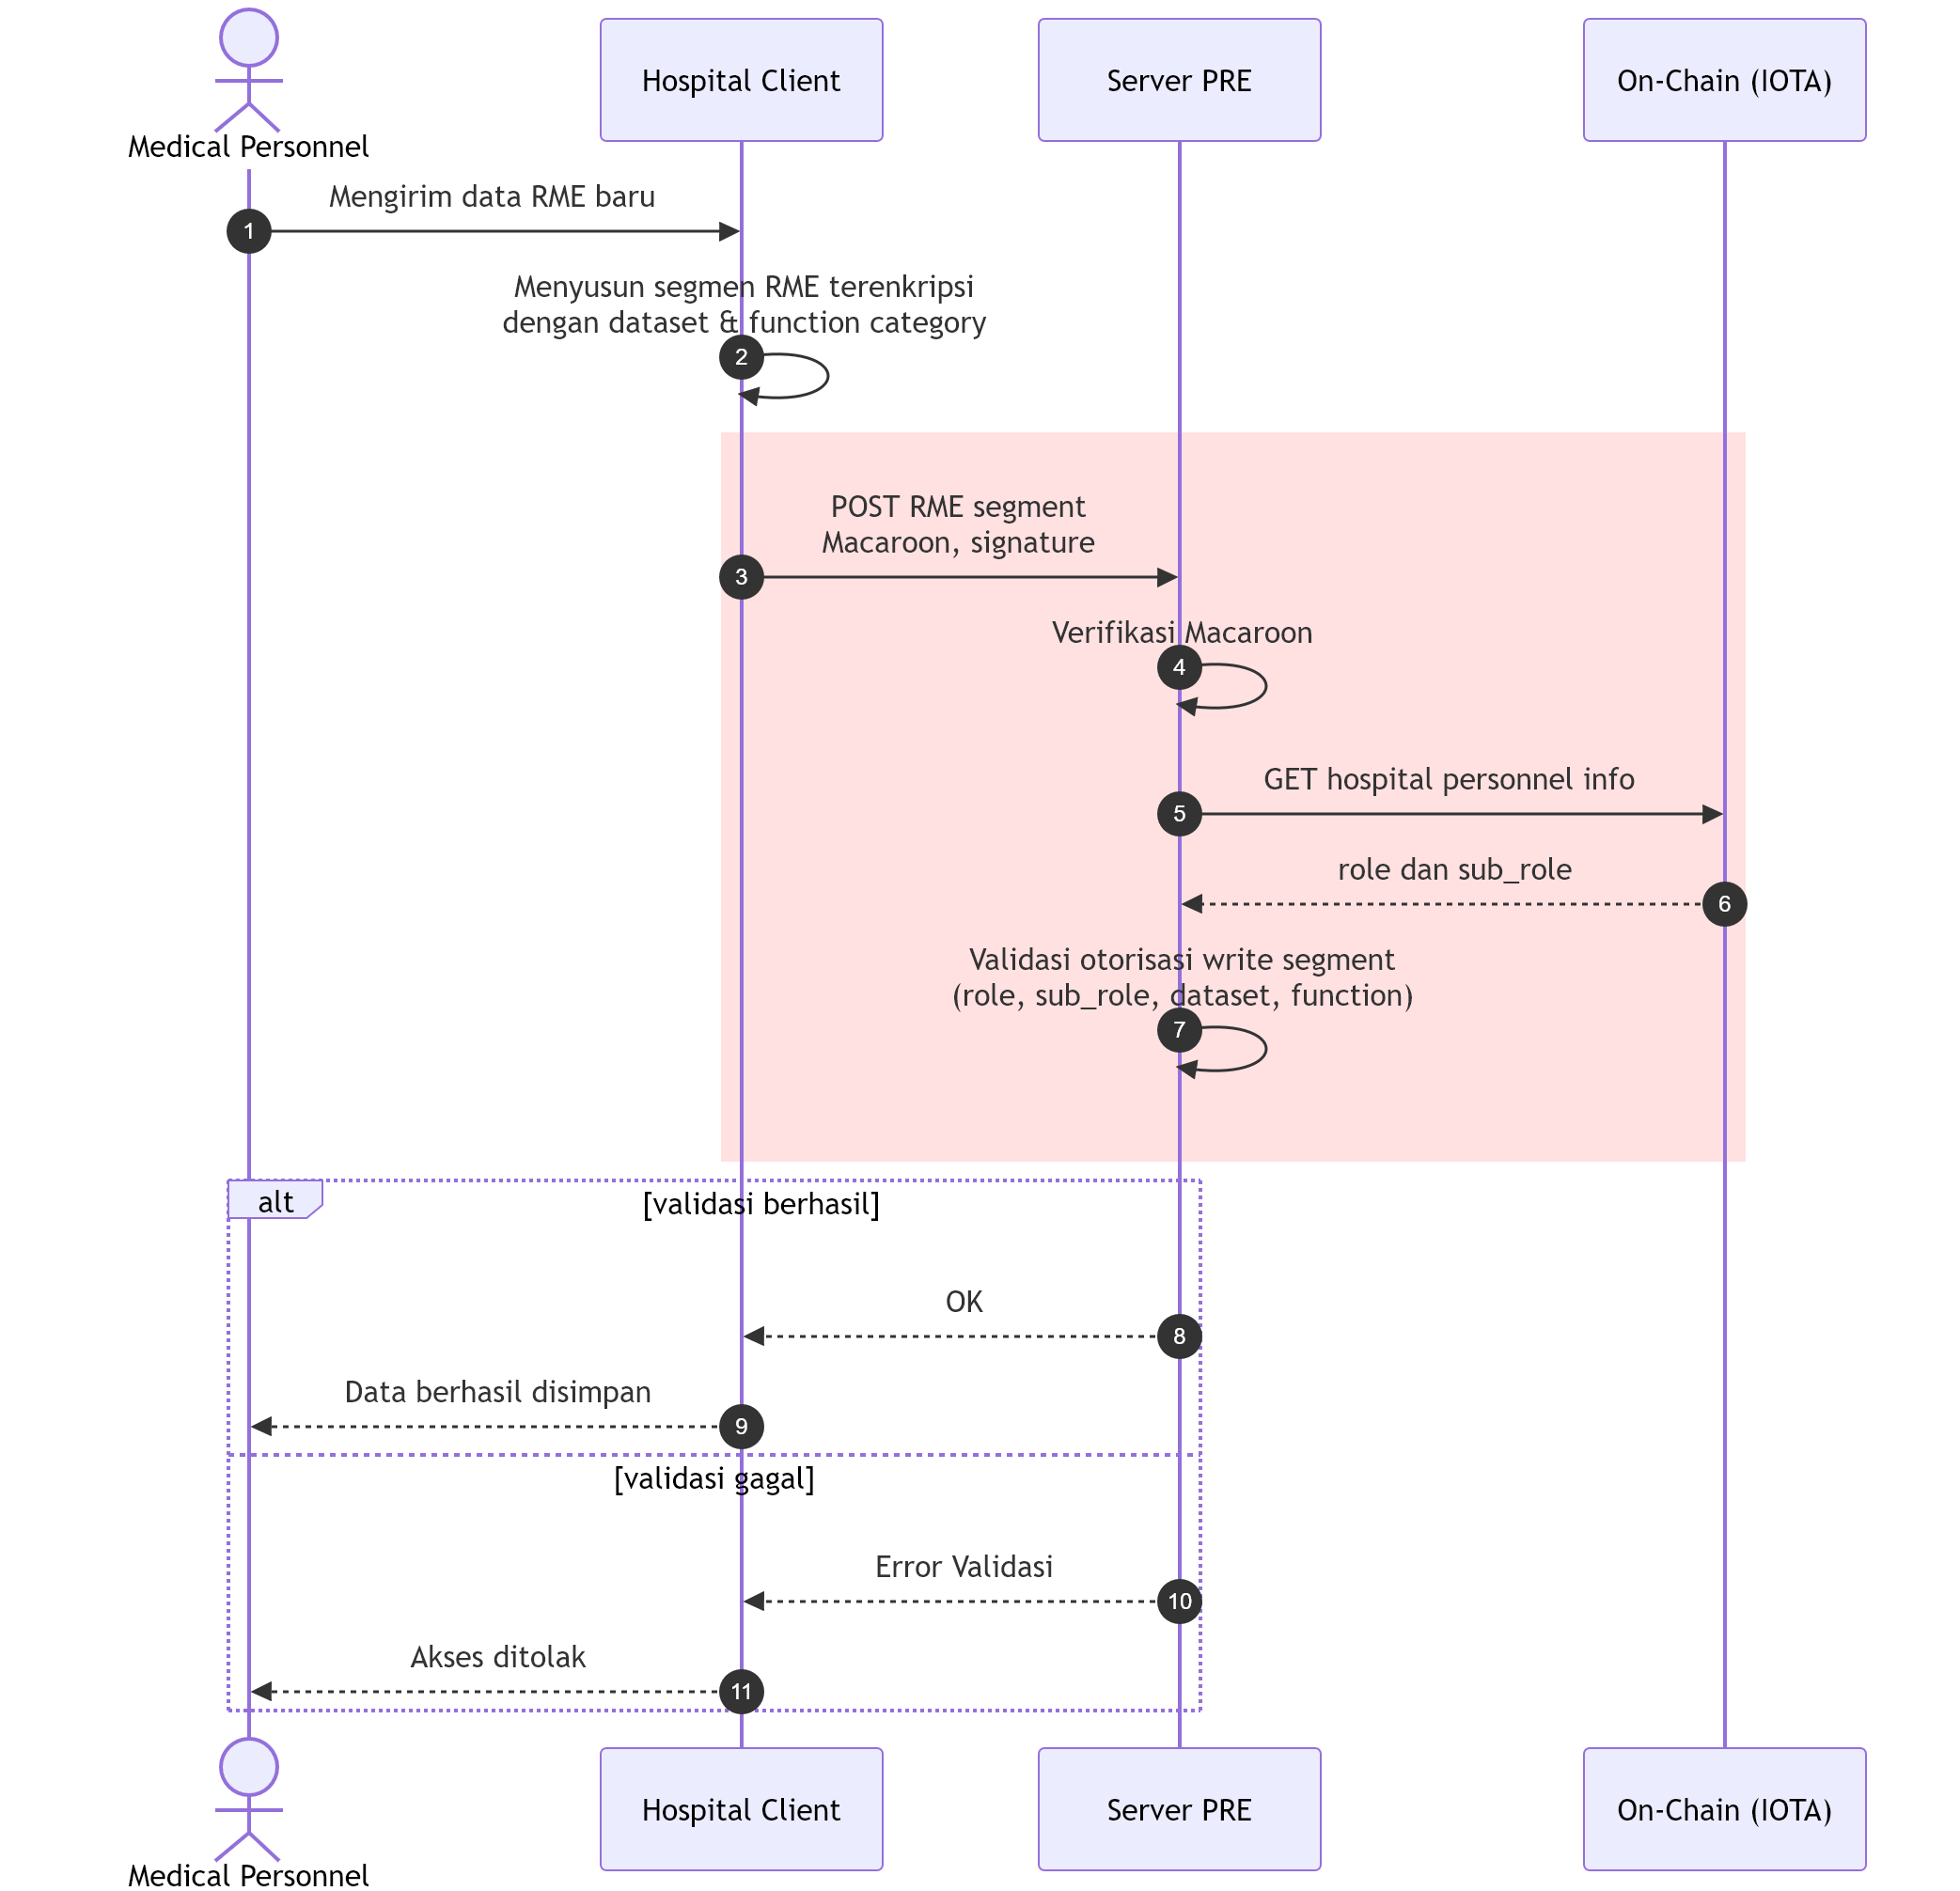
\includegraphics[width=0.95\textwidth,height=0.80\textheight,keepaspectratio]{resources/chapter-3/rancangan/seqdiag-validasi-subrole X dataset.png}
	\caption{\textit{Sequence Diagram} Rancangan Validasi \textit{subrole} Tenaga Medis terhadap \textit{Dataset Category}}
	\label{fig:seqdiag-validasi-subrole-dataset}
\end{figure}

Validasi menggunakan data \textit{role} dan \textit{subrole} yang terdapat pada penyimpanan\textit{on-chain} karena pada Macaroon tidak terdapat informasi \textit{role} dari pengguna aktif saat ini, sesuai dengan rancangan \textit{caveats} pada Tabel \ref{tab:rancangan-caveats-macaroons-baru}. Sementara itu, \textit{registry personnel} pada penyimpanan \textit{on-chain} merepresentasikan status kelembagaan aktor, misalnya apakah aktor masih terdaftar sebagai \textit{personnel} rumah sakit dengan \textit{role} atau \textit{subrole} tertentu. Dengan demikian, \textit{request} hanya dilanjutkan apabila aktor memiliki token yang valid sekaligus masih memiliki otoritas kelembagaan yang sesuai.

\subsubsection{Verifikasi \textit{Wallet} Aktor Aktif}
\label{subsubsec:verifikasi-wallet-aktor-aktif}

Sesuai analisis pada Subbab \ref{subsec:verifikasi-bukti-kepemilikan-wallet}, diperlukan verifikasi tambahan terhadap \textit{wallet} aktor aktif untuk memastikan \textit{request} dilakukan oleh aktor aktif yang sah.

Rancangan proses verifikasi dilakukan dengan mekanisme \textit{presigned request}. Ketika \textit{client} mengirimkan \textit{request} ke \textit{Server} PRE, \textit{client} juga menambahkan header yang berisi konteks \textit{request} yang telah di-\textit{sign} menggunakan kunci privat \textit{wallet} pengguna. Konteks \textit{request} memuat informasi seperti \texttt{token\_id}, \texttt{patient\_address}, \texttt{related\_rme\_id}, \texttt{operation}, \texttt{segment\_id}, \texttt{dataset\_category}, \texttt{function\_category}, dan \texttt{timestamp}. Keberadaan \textit{timestamp} pada konteks yang ditandatangani juga membuat \textit{signature} hanya berlaku untuk rentang waktu tertentu. Apabila \textit{signature} tidak valid maka \textit{request} ditolak.

\subsubsection{Pencabutan Hak Akses Macaroon Delegasi}
\label{subsubsec:pencabutan-hak-akses-macaroon-delegasi}

Sesuai dengan analisis pada Subbab \ref{subsec:analisis-revokasi-audit-delegasi}, diperlukan mekanisme revokasi dan audit delegasi untuk memastikan bahwa pencabutan akses dapat berdampak pada seluruh token turunan yang berasal dari token tersebut. Revokasi akses pada implementasi Tugas Akhir ini masih menjadikan pasien sebagai \textit{resource owner} yang berwenang untuk mencabut akses terhadap RME.

Revokasi akses pada implementasi ini dilakukan melalui kombinasi pencatatan status di IOTA \textit{on-chain} dan Redis PRE, dengan \textit{server} PRE bertindak sebagai titik penegakan kebijakan akses. Lapisan \textit{on-chain} digunakan untuk mencatat perubahan status akses dan audit trail revokasi, sedangkan Redis PRE digunakan untuk menyimpan \textit{hash} dari token yang telah dicabut. Alur pencabutan akses oleh pasien ditunjukkan pada Gambar \ref{fig:seqdiag-revoke-access}. Pada alur tersebut, pasien memilih akses yang akan dicabut melalui \textit{Patient Client}. \textit{Patient Client} kemudian mengeksekusi fungsi \texttt{revoke\_access()} pada \textit{smart contract} Move untuk menandai akses sebagai dicabut, menghapus hak akses pada penyimpanan \textit{on-chain}, melakukan pencabutan berantai terhadap penerima delegasi turunan, serta mencatat kejadian revokasi ke dalam \textit{audit log}. Setelah transaksi \textit{on-chain} berhasil, \textit{Patient Client} mengirimkan \textit{payload} revokasi ke \textit{Server} PRE agar menyimpan \textit{hash} dari token yang telah dicabut pada Redis PRE dan menghapus \textit{re-encryption key} terkait dengan token Macaroon yang direvokasi.

\begin{figure}[!ht]
	\centering
	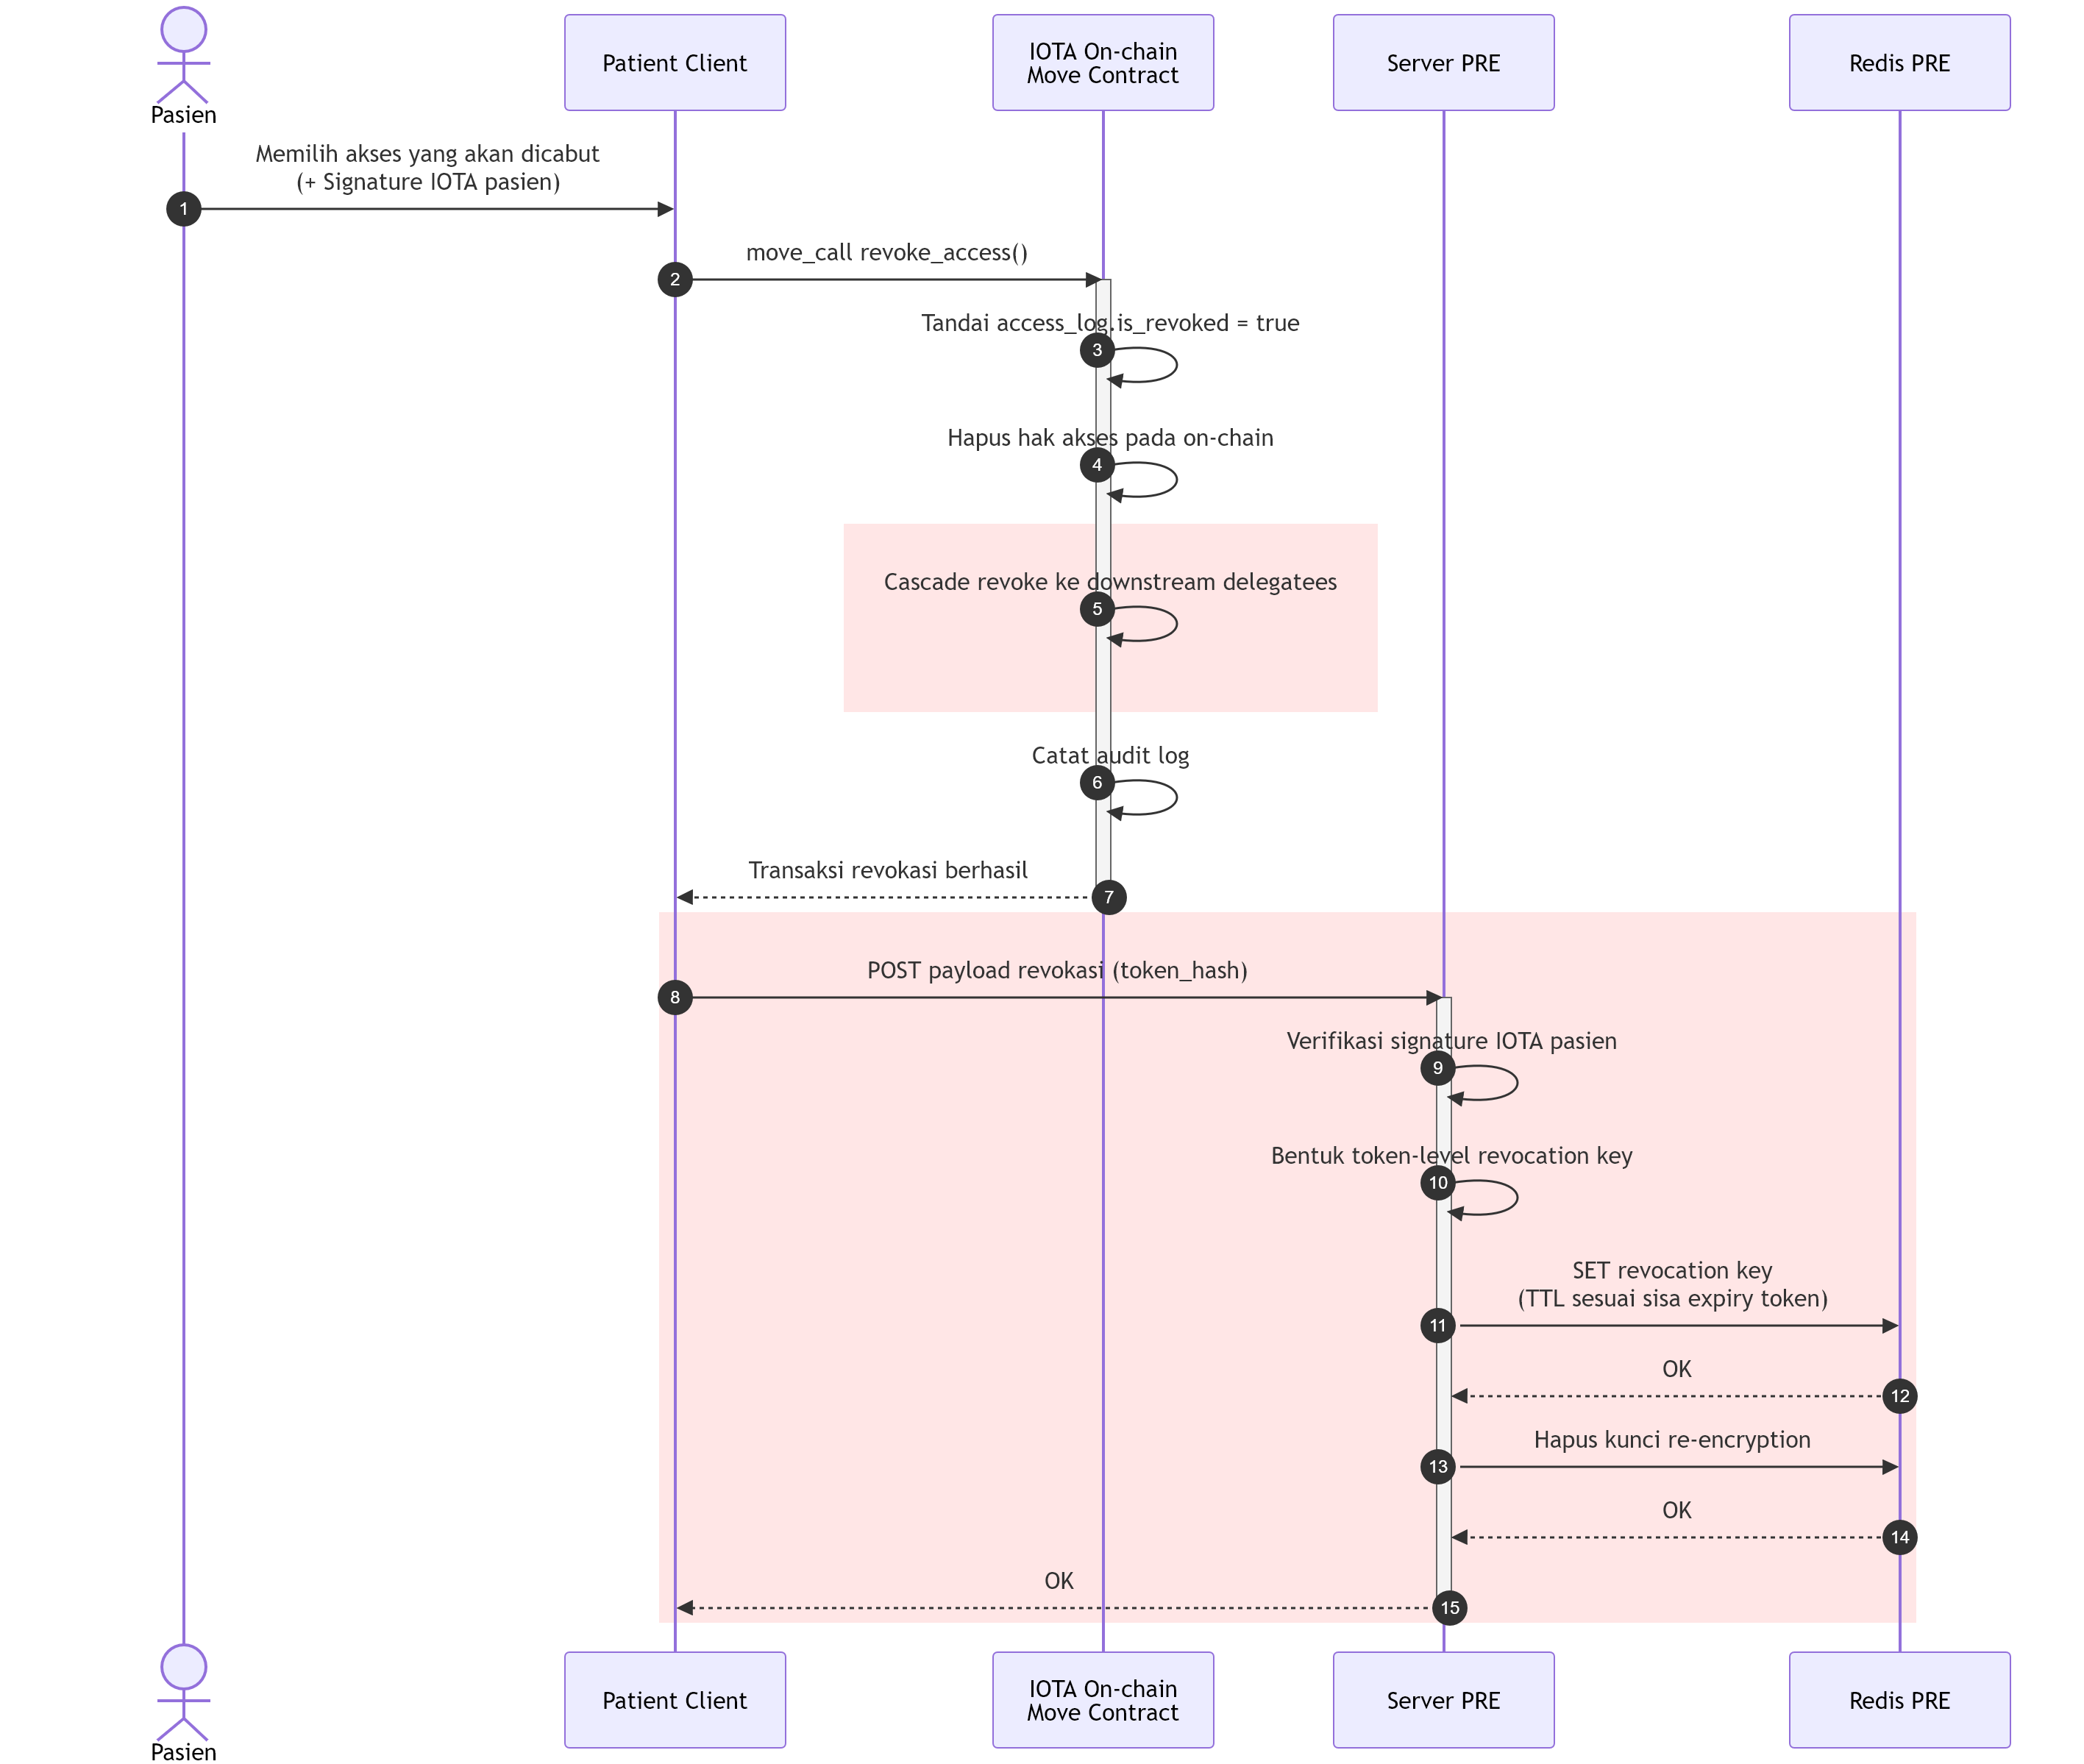
\includegraphics[width=0.95\textwidth,height=0.80\textheight,keepaspectratio]{resources/chapter-3/rancangan/seqdiag-revoke_access.png}
	\caption{\textit{Sequence Diagram} Rancangan Alur Pencabutan Hak Akses Macaroon Delegasi}
	\label{fig:seqdiag-revoke-access}
\end{figure}

Bagian berlatar merah pada Gambar \ref{fig:seqdiag-revoke-access} menunjukkan alur baru yang ditambahkan pada Tugas Akhir ini. Alur baru tersebut mencakup pencabutan berantai terhadap seluruh \textit{downstream delegatees}, pengiriman \textit{payload} revokasi ke \textit{Server} PRE, pembentukan \textit{revocation key}, penyimpanan status revokasi pada Redis dengan TTL sesuai masa berlaku token, serta penghapusan kunci \textit{re-encryption}. Dengan penambahan alur ini, revokasi tidak hanya tercatat pada IOTA, tetapi juga langsung ditegakkan oleh \textit{Server} PRE ketika token Macaroon digunakan kembali.

Pada saat verifikasi, \textit{Server} PRE memeriksa \textit{hash} token yang sedang digunakan dan setiap \textit{caveat} \texttt{parent\_token\_hash} ke \textit{revocation key} pada Redis.  Dengan demikian, apabila pasien mencabut akses pada delegator awal, maka token Macaroon turunan yang dibuat dari akses tersebut juga akan dianggap tidak valid. Selain itu, pemerikskaan status hak akses juga dilakukan pada penyimpanan \textit{on-chain} yang mencatat status hak akses.
\subsection{Rancangan Alur Akses dan Delegasi}
\label{subsec:rancangan-alur-akses-dan-delegasi}

Fitur \textit{offline attenuation} dirancang untuk menjawab kebutuhan delegasi akses antar tenaga medis tanpa mengharuskan pasien menerbitkan ulang token setiap kali terjadi perpindahan tugas. Pada rancangan ini, istilah \textit{offline} tidak berarti bahwa seluruh proses akses data dilakukan tanpa koneksi ke \textit{Server} PRE. Istilah tersebut merujuk pada kemampuan pemegang token untuk menurunkan atau mengatenuasi token secara lokal pada aplikasi \textit{client}, tanpa meminta \textit{Server} PRE menerbitkan token baru.

Delegasi akses pada rancangan ini terdiri atas dua tahap utama. Tahap pertama adalah delegasi awal dari pasien kepada dokter penanggung jawab pasien. Pada tahap ini, pasien memberikan persetujuan akses, kemudian \textit{Server} PRE menerbitkan token Macaroon awal untuk dokter. Tahap kedua adalah delegasi lanjutan dari dokter kepada aktor layanan kesehatan lain, seperti perawat, petugas laboratorium, atau apoteker. Pada tahap kedua ini, token tidak diterbitkan ulang oleh \textit{Server} PRE, melainkan diturunkan secara lokal oleh aplikasi \textit{client} dokter dengan menambahkan \textit{caveats} baru yang lebih ketat.

Macaroons mendukung atenuasi lokal karena token turunan dapat dibuat dengan menambahkan \textit{caveats} baru pada token induk. Penambahan \textit{caveats} menghasilkan tanda tangan Macaroon baru melalui mekanisme \textit{chained-HMAC}. Karena \textit{caveats} pada Macaroon bersifat \textit{append-only}, token turunan tidak dapat menghapus batasan pada token induk. Dengan demikian, token turunan hanya dapat memiliki cakupan akses yang sama atau lebih sempit daripada token induknya.

\subsubsection{Delegasi Awal dari Pasien kepada Dokter}

Delegasi awal merupakan proses pemberian otorisasi pertama dari pasien kepada dokter penanggung jawab pasien. Pada tahap ini, pasien tetap menjadi pihak yang mengendalikan pemberian akses awal terhadap data RME miliknya. Namun, karena \texttt{RootKey} Macaroon hanya dimiliki oleh \textit{Server} PRE, pasien tidak membuat token Macaroon secara langsung. Pasien memberikan persetujuan melalui \textit{Patient Client}, kemudian \textit{Server} PRE menerbitkan token awal berdasarkan persetujuan tersebut.

Alur delegasi awal dari pasien kepada dokter adalah sebagai berikut.

\begin{enumerate}[leftmargin=*]
	\item Pasien memilih konteks jenis pelayanan kesehatan dan melakukan scan kode QR yang berisi data	\texttt{iota\_address} dan \texttt{pre\_public\_key} dari dokter penanggung jawab pasien.
	\item Pasien menentukan konteks layanan kesehatan, misalnya rawat jalan.
	\item \textit{Patient Client} mengirimkan permintaan penerbitan token kepada \textit{Server} PRE.
	\item \textit{Server} PRE memvalidasi identitas pasien dan cakupan akses yang diminta.
	\item \textit{Server} PRE menerbitkan Macaroon awal dengan \textit{caveats} yang mengikat token pada pasien, RME terkait, dokter penerima akses, cakupan baca dan tulis, masa berlaku, serta batas kedalaman delegasi.
	\item Token awal diberikan kepada dokter melalui \textit{Hospital Client} atau disimpan pada penyimpanan token aplikasi yang hanya dapat diakses oleh dokter terkait.
\end{enumerate}

Contoh \textit{caveats} pada token awal yang diberikan kepada dokter dalam konteks pelayanan rawat jalanditunjukkan pada Listing \ref{lst:caveat-token-awal-dokter}.

\begin{lstlisting}[caption={Contoh \textit{Caveats} Token Awal dari Pasien kepada Dokter}, label={lst:caveat-token-awal-dokter}]
patient_address = 0xPASIEN
related_rme_id = RME-001
root_subject = 0xDOKTER

read_dataset_in = [RAWAT_JALAN, LABORATORIUM, APOTEK]
write_dataset_in = [RAWAT_JALAN, LABORATORIUM, APOTEK]

read_function_in = [
  ANAMNESIS,
  PEMERIKSAAN_FISIK,
  PEMERIKSAAN_PSIKOLOGIS,
  DIAGNOSIS,
  TERAPI,
  PERMINTAAN_PEMERIKSAAN,
  HASIL_PEMERIKSAAN,
  DATA_RESEP_DAN_OBAT
]

write_function_in = [
  ANAMNESIS,
  PEMERIKSAAN_FISIK,
  DIAGNOSIS,
  TERAPI,
  PERMINTAAN_PEMERIKSAAN
]

expires_before = 2026-05-16T18:00:00
max_delegation_depth = 1
\end{lstlisting}

Pada contoh tersebut, \texttt{root\_subject} menyatakan bahwa dokter merupakan penerima token awal. \texttt{patient\_address} mengikat token pada data pasien tertentu, sedangkan \texttt{related\_rme\_id} membatasi token pada episode RME tertentu. \texttt{read\_dataset\_in}, \texttt{write\_dataset\_in}, \texttt{read\_function\_in}, dan \texttt{write\_function\_in} menyatakan cakupan akses yang diberikan. \texttt{expires\_before} membatasi masa berlaku token. Sementara itu, \texttt{max\_delegation\_depth} membatasi jumlah delegasi lanjutan yang dapat dilakukan dari token tersebut.

\subsubsection{Delegasi Lokal dari Dokter kepada Aktor Lain}

Setelah dokter menerima token awal, dokter dapat menurunkan token tersebut kepada aktor layanan kesehatan lain apabila dibutuhkan dalam proses pelayanan. Delegasi ini dilakukan secara lokal pada aplikasi \textit{client} dokter dengan menambahkan \textit{caveats} baru pada token induk. \textit{Server} PRE tidak menerbitkan token baru pada tahap ini.

Aktor yang dapat menerima token turunan dari dokter mencakup perawat, petugas laboratorium, dan apoteker. Setiap aktor hanya menerima cakupan akses sesuai kebutuhan tugasnya. Contoh pemetaan kebutuhan delegasi ditunjukkan pada Tabel \ref{tab:pemetaan-delegasi-dokter}.

\begin{table}[!ht]
	\centering
	\caption{Pemetaan Delegasi Token dari Dokter kepada Aktor Lain}
	\label{tab:pemetaan-delegasi-dokter}
	\small
	\begin{tabular}{|p{0.18\textwidth}|p{0.23\textwidth}|p{0.43\textwidth}|}
		\hline
		\textbf{Penerima Delegasi} & \textbf{Tujuan Delegasi}                                                                                                                                             & \textbf{Cakupan Akses} \\ \hline

		Perawat
		                           & Membantu pengisian dan pembacaan data klinis tertentu.
		                           & Membaca dan/atau menulis segmen seperti anamnesis, pemeriksaan fisik, pemeriksaan psikologis, serta instruksi medik dan keperawatan sesuai kebutuhan layanan.
		\\ \hline

		Petugas laboratorium
		                           & Memproses permintaan pemeriksaan dan mengunggah hasil laboratorium.
		                           & Membaca segmen permintaan pemeriksaan dan menulis segmen hasil pemeriksaan pada \textit{dataset} laboratorium.
		\\ \hline

		Apoteker
		                           & Memproses resep dan penyerahan obat.
		                           & Membaca segmen resep, alergi, dan informasi obat yang relevan, serta menulis status pengkajian resep, status resep, waktu penyiapan obat, dan waktu penyerahan obat.
		\\ \hline
	\end{tabular}
\end{table}

Sebagai contoh, apabila dokter membutuhkan pemeriksaan laboratorium, aplikasi \textit{client} dokter membuat token turunan untuk petugas laboratorium dengan menambahkan \textit{caveats} baru seperti pada Listing \ref{lst:caveat-token-turunan-lab}.

\begin{lstlisting}[caption={Contoh \textit{Caveats} Tambahan Token Turunan untuk Petugas Laboratorium}, label={lst:caveat-token-turunan-lab}]
delegated_by = 0xDOKTER
delegated_to = 0xLAB

read_dataset_in = [LABORATORIUM]
write_dataset_in = [LABORATORIUM]

read_function_in = [PERMINTAAN_PEMERIKSAAN]
write_function_in = [HASIL_PEMERIKSAAN]

expires_before = 2026-05-16T14:00:00
max_delegation_depth = 1
\end{lstlisting}

Pada contoh tersebut, token turunan hanya dapat digunakan oleh petugas laboratorium untuk membaca permintaan pemeriksaan dan menulis hasil pemeriksaan. Token tidak dapat digunakan untuk membaca diagnosis, anamnesis, terapi, resep, atau segmen klinis lain yang tidak termasuk dalam \textit{caveats} token turunan.

Nilai \texttt{max\_delegation\_depth} pada rancangan ini diperlakukan sebagai batas maksimum panjang rantai delegasi, bukan sebagai nilai yang ditimpa secara bebas. \textit{Server} PRE menghitung jumlah \textit{caveat} \texttt{delegated\_to} pada token untuk menentukan kedalaman delegasi aktual. Apabila token awal memiliki \texttt{max\_delegation\_depth = 1}, maka token tersebut hanya boleh diturunkan satu kali dari dokter kepada aktor lain. Jika aktor penerima mencoba menurunkan token lagi kepada pihak berikutnya, jumlah delegasi akan melebihi batas dan token ditolak oleh \textit{Server} PRE.

\subsubsection{Proses Pemberian Token Turunan}

Proses pemberian token turunan dari dokter kepada aktor lain tidak dilakukan dengan meminta \textit{Server} PRE membuat token baru. Dokter menurunkan token secara lokal, kemudian token turunan diberikan kepada aktor penerima melalui kanal aplikasi yang terautentikasi, misalnya melalui \textit{Hospital Client} atau penyimpanan token internal yang dikelola oleh sistem.

Agar proses delegasi dapat diaudit dan tidak bergantung hanya pada isi token, aplikasi dokter juga membuat bukti delegasi yang ditandatangani menggunakan kunci privat \textit{wallet} dokter. Bukti ini digunakan untuk menunjukkan bahwa token turunan benar-benar dibuat oleh pihak yang dinyatakan pada \texttt{delegated\_by}. Bukti delegasi dapat disertakan sebagai metadata pendamping token atau dicatat sebagai \textit{event} pada sistem.

Struktur konseptual pemberian token turunan ditunjukkan pada Listing \ref{lst:delegation-envelope}.

\begin{lstlisting}[caption={Struktur Konseptual Pemberian Token Turunan}, label={lst:delegation-envelope}]
DelegationEnvelope {
  macaroon_token: "<attenuated_macaroon>",
  delegated_by: "0xDOKTER",
  delegated_to: "0xLAB",
  related_rme_id: "RME-001",
  issued_at: "2026-05-16T10:30:00",
  expires_before: "2026-05-16T14:00:00",
  token_hash: "hash(attenuated_macaroon)",
  delegation_signature: "signature_by_0xDOKTER"
}
\end{lstlisting}

\texttt{delegation\_signature} merupakan tanda tangan digital dari dokter terhadap konteks delegasi, misalnya \texttt{delegated\_to}, \texttt{related\_rme\_id}, \texttt{expires\_before}, dan \texttt{token\_hash}. Dengan demikian, pihak lain yang hanya memperoleh token dokter secara tidak sah tidak dapat membuat delegasi yang valid atas nama dokter tanpa memiliki kunci privat \textit{wallet} dokter.

Secara umum, proses pemberian token turunan berlangsung sebagai berikut.

\begin{enumerate}[leftmargin=*]
	\item Dokter memilih aktor penerima delegasi melalui \textit{Hospital Client}, misalnya petugas laboratorium.
	\item Aplikasi dokter menentukan cakupan akses yang akan diberikan, seperti \texttt{LABORATORIUM} dan \texttt{HASIL\_PEMERIKSAAN}.
	\item Aplikasi dokter menambahkan \textit{caveats} baru ke Macaroon induk sehingga terbentuk Macaroon turunan.
	\item Aplikasi dokter menghitung \textit{hash} dari Macaroon turunan.
	\item Dokter menandatangani konteks delegasi menggunakan kunci privat \textit{wallet}.
	\item Macaroon turunan beserta bukti delegasi dikirimkan kepada aktor penerima melalui kanal aplikasi yang terautentikasi.
	\item Aktor penerima menyimpan token turunan dan menggunakannya ketika membutuhkan akses ke segmen RME terkait.
\end{enumerate}

\subsubsection{Contoh Delegasi kepada Perawat, Laboratorium, dan Apotek}

Contoh \textit{caveats} tambahan untuk token turunan kepada perawat ditunjukkan pada Listing \ref{lst:caveat-token-turunan-perawat}.

\begin{lstlisting}[caption={Contoh \textit{Caveats} Tambahan Token Turunan untuk Perawat}, label={lst:caveat-token-turunan-perawat}]
delegated_by = 0xDOKTER
delegated_to = 0xPERAWAT

read_dataset_in = [RAWAT_JALAN]
write_dataset_in = [RAWAT_JALAN]

read_function_in = [
  ANAMNESIS,
  PEMERIKSAAN_FISIK,
  PEMERIKSAAN_PSIKOLOGIS,
  INSTRUKSI_MEDIK_DAN_KEPERAWATAN
]

write_function_in = [
  ANAMNESIS,
  PEMERIKSAAN_FISIK,
  PEMERIKSAAN_PSIKOLOGIS
]

expires_before = 2026-05-16T16:00:00
max_delegation_depth = 1
\end{lstlisting}

Contoh \textit{caveats} tambahan untuk token turunan kepada apoteker ditunjukkan pada Listing \ref{lst:caveat-token-turunan-apoteker}.

\begin{lstlisting}[caption={Contoh \textit{Caveats} Tambahan Token Turunan untuk Apoteker}, label={lst:caveat-token-turunan-apoteker}]
delegated_by = 0xDOKTER
delegated_to = 0xAPOTEKER

read_dataset_in = [APOTEK]
write_dataset_in = [APOTEK]

read_function_in = [
  DATA_RESEP_DAN_OBAT,
  RIWAYAT_ALERGI,
  ASAL_RESEP,
  DOKTER_PENULIS_RESEP
]

write_function_in = [
  STATUS_DAN_PENGKAJIAN_RESEP,
  STATUS_RESEP,
  WAKTU_PENYIAPAN_OBAT,
  WAKTU_PENYERAHAN_OBAT,
  PETUGAS_DISPENSING
]

expires_before = 2026-05-16T17:00:00
max_delegation_depth = 1
\end{lstlisting}

Pada kedua contoh tersebut, token turunan tetap membawa seluruh \textit{caveats} dari token dokter. Oleh karena itu, apabila token dokter hanya berlaku untuk \texttt{related\_rme\_id = RME-001}, maka token perawat, token laboratorium, dan token apoteker juga hanya berlaku untuk RME tersebut. Apabila token dokter berlaku sampai pukul 18.00, token turunan tidak dapat memperpanjang masa berlaku melebihi waktu tersebut karena \textit{Server} PRE akan memvalidasi seluruh \textit{caveats} \texttt{expires\_before} dan menggunakan batas waktu yang paling ketat.

\subsubsection{Verifikasi Token Turunan oleh \textit{Server} PRE}

Ketika aktor penerima delegasi menggunakan token turunan, \textit{Server} PRE bertindak sebagai titik penegakan kebijakan akses. \textit{Server} PRE tidak menerbitkan ulang token, tetapi memverifikasi token turunan dan seluruh bukti yang menyertainya.

Langkah verifikasi token turunan adalah sebagai berikut.

\begin{enumerate}[leftmargin=*]
	\item \textit{Server} PRE memverifikasi validitas Macaroon menggunakan \texttt{RootKey}.
	\item \textit{Server} PRE memverifikasi bahwa \texttt{patient\_address} dan \texttt{related\_rme\_id} pada token sesuai dengan data RME yang diminta.
	\item \textit{Server} PRE menghitung aktor aktif. Jika tidak terdapat \texttt{delegated\_to}, maka aktor aktif adalah \texttt{root\_subject}. Jika terdapat satu atau lebih \texttt{delegated\_to}, maka aktor aktif adalah nilai \texttt{delegated\_to} terakhir.
	\item \textit{Server} PRE memverifikasi tanda tangan \textit{wallet} dari aktor aktif pada permintaan akses.
	\item \textit{Server} PRE memverifikasi bukti delegasi dari pihak yang dinyatakan pada \texttt{delegated\_by}.
	\item \textit{Server} PRE menghitung kedalaman delegasi berdasarkan jumlah \texttt{delegated\_to} pada token dan memastikan nilainya tidak melebihi \texttt{max\_delegation\_depth}.
	\item \textit{Server} PRE memvalidasi seluruh batas waktu pada \texttt{expires\_before} dan menggunakan batas waktu yang paling awal sebagai masa berlaku efektif token.
	\item \textit{Server} PRE menghitung cakupan akses efektif berdasarkan irisan seluruh \texttt{read\_dataset\_in}, \texttt{write\_dataset\_in}, \texttt{read\_function\_in}, dan \texttt{write\_function\_in}.
	\item \textit{Server} PRE mengambil metadata segmen dari IOTA dan mencocokkan \texttt{dataset\_category} serta \texttt{function\_category} segmen dengan cakupan akses efektif token.
	\item Jika seluruh verifikasi berhasil, \textit{Server} PRE melanjutkan proses pengambilan data terenkripsi dari IPFS dan melakukan \textit{re-encryption}. Jika salah satu pemeriksaan gagal, permintaan akses ditolak.
\end{enumerate}

Dengan mekanisme tersebut, token turunan tidak dapat memperluas hak akses token induk. Misalnya, apabila token dokter tidak memiliki akses terhadap \texttt{APOTEK}, maka dokter tidak dapat membuat token turunan yang valid untuk apoteker. Meskipun dokter menambahkan \textit{caveat} \texttt{read\_dataset\_in = [APOTEK]}, cakupan efektif token akan menjadi kosong karena batasan tersebut tidak termasuk dalam cakupan token induk. Demikian pula, apabila token dokter hanya berlaku hingga pukul 18.00, token turunan yang mencoba menggunakan \texttt{expires\_before} setelah pukul 18.00 tetap tidak akan memperpanjang masa berlaku efektif token.

Rancangan ini mempertahankan kendali awal pasien karena token awal tetap diterbitkan berdasarkan persetujuan pasien. Pada saat yang sama, rancangan ini mengurangi hambatan operasional pada pelayanan klinis karena dokter dapat menurunkan token secara lokal kepada aktor lain yang terlibat dalam layanan. Dengan demikian, mekanisme delegasi ini mendukung kolaborasi layanan kesehatan yang dinamis, menjaga prinsip \textit{least privilege}, dan tetap mempertahankan peran \textit{Server} PRE sebagai titik verifikasi dan penegakan akses.
% \subsection{Rancangan Client}
\label{subsec:rancangan-client}

Rancangan client tidak menjadi bagian dari rancangan solusi utama, melainkan menjadi implikasi dari rancangan solusi yang telah diuraikan pada subbab sebelumnya.

Pada DecMed, terdapat tiga \textit{client} utama, yaitu \textit{Patient Client}, \textit{Hospital Client}, dan \textit{Ministry Client}. Perubahan pada rancangan \textit{client} hanya dibutuhkan pada \textit{Patient Client} dan \textit{Hospital Client}.

\subsubsection{Rancangan \textit{Patient Client}}
\label{subsubsec:rancangan-patient-client}

Perubahan pada \textit{Patient Client} dibutuhkan pada halaman berikut:

\begin{itemize}
	\item Halaman Home (List RME) disesuaikan agar tetap menampilkan daftar RME milik pasien, namun yang dibaca adalah segmen-segmen data yang dikelompokkan.
	\item Halaman Detail RME tetap menampilkan detail RME milik pasien, namun yang dibaca adalah segmen-segmen data RME. Data dikelompokkan berdasarkan \textit{dataset category}.
	\item Halaman Audit Delegasi merupakan halaman baru yang menampilkan informasi mengenai seluruh rantai delegasi akses yang terbentuk dari token Macaroon yang telah diterbitkan oleh pasien.
	      % \item Halaman Log Akses disesuaikan agar tetap menampilkan log akses milik pasien, namun yang dibaca adalah log akses yang terkait delegasi Macaroons.
	\item Halaman \textit{Scan} QR disesuaikan dengan menambahkan form untuk menentukan batasan akses yang akan diberikan.
\end{itemize}

\subsubsection{Rancangan \textit{Hospital Client}}
\label{subsubsec:rancangan-hospital-client}

Perubahan pada \textit{Hospital Client} dibutuhkan pada halaman berikut:

\begin{itemize}
	\item Halaman \textit{Dashboard} disesuaikan agar tetap menampilkan daftar akses yang dimiliki \textit{personnel} sesuai token yang dimiliki.
	\item Halaman Delegasi Akses merupakan halaman baru yang menampilkan informasi mengenai seluruh rantai delegasi akses yang terbentuk dari token Macaroon yang telah diterbitkan oleh pasien.
	\item Halaman Daftar RME pasien disesuaikan agar tetap menampilkan daftar RME milik pasien, namun sudah dikelompokan per episode RME.
	\item Halaman Detail RME disesuaikan agar tetap menampilkan detail RME milik pasien, namun yang dibaca adalah segmen-segmen data yang dikelompokkan.
	\item Halaman penulisan segmenRME disesuaikan agar tetap menampilkan form untuk menulis segmen RME milik pasien, namun yang ditulis adalah segmen-segmen data yang dikelompokkan.
\end{itemize}

\subsection{Pemetaan Rancangan terhadap Solusi}
\label{subsec:pemetaan-rancangan-solusi}

Setelah rancangan solusi diuraikan, setiap rancangan dipetakan kembali terhadap solusi yang telah dianalisis pada Subbab \ref{subsec:pemetaan-kebutuhan-solusi}. Melalui pemetaan ini, keterkaitan langsung setiap rancangan \texttt{R-TA} dengan solusi \texttt{S-TA} yang diusulkan ditunjukkan. Hasil pemetaan rancangan terhadap solusi ditunjukkan pada Tabel \ref{tab:daftar-rancangan-solusi}.

\begin{table}[!ht]
	\centering
	\caption{Pemetaan Rancangan terhadap Solusi}
	\label{tab:daftar-rancangan-solusi}
	\small
	\begin{tabular}{|p{0.12\textwidth}|p{0.54\textwidth}|p{0.24\textwidth}|}
		\hline
		\textbf{ID}      & \textbf{Nama Rancangan}                                                                                                                            & \textbf{Merealisasikan Solusi}                                         \\ \hline
		\texttt{R-TA-01} & Rancangan arsitektur solusi DecMed dengan PBAC, Macaroons, segmentasi, dan PRE sebagai \textit{policy enforcement point}.                  & \texttt{S-TA-01}, \texttt{S-TA-02}, \texttt{S-TA-03}, \texttt{S-TA-04} \\ \hline
		\texttt{R-TA-02} & Rancangan segmentasi data RME berdasarkan \textit{dataset} dan \textit{function category}.                                                         & \texttt{S-TA-02}                                                       \\ \hline
		\texttt{R-TA-03} & Rancangan model PBAC pada DecMed.                                                                                                                  & \texttt{S-TA-01}                                                       \\ \hline
		\texttt{R-TA-04} & Rancangan representasi kapabilitas pada \textit{caveats} Macaroons dan rantai delegasi.                                                            & \texttt{S-TA-03}                                                       \\ \hline
		\texttt{R-TA-05} & Rancangan penegakan kebijakan akses berdasarkan kapabilitas efektif token Macaroon dan bukti kepemilikan \textit{wallet} pada \textit{Server} PRE. & \texttt{S-TA-01}, \texttt{S-TA-04}                                     \\ \hline
		\texttt{R-TA-06} & Rancangan validasi \textit{subrole} tenaga medis terhadap \textit{dataset category}.                                                               & \texttt{S-TA-05}                                                       \\ \hline
		\texttt{R-TA-07} & Rancangan revokasi delegasi token Macaroons.                                                                                                       & \texttt{S-TA-06}                                                       \\ \hline
		\texttt{R-TA-08} & Rancangan alur akses dan delegasi pada skenario layanan kesehatan kolaboratif.                                                                     & \texttt{S-TA-03}, \texttt{S-TA-04}, \texttt{S-TA-05}                   \\ \hline
	\end{tabular}
\end{table}
